\documentclass[12pt]{article}
\usepackage{setspace}

\setlength{\headheight}{35pt} 

\usepackage[hang,flushmargin]{footmisc}
\usepackage[vmargin=1in,hmargin=1.1in]{geometry}				% page layout
%\usepackage{geometry}	
\usepackage{amssymb,amsmath,amsfonts,amsthm,mathtools,bm,bbm,mathrsfs} 	% math fonts/symbols
\usepackage[dvipsnames]{xcolor} 								% for \textcolor
\usepackage[hidelinks]{hyperref} 								% for hyperlinks 
\usepackage{graphicx} 											% for \includegraphics
\usepackage{caption} 											% for figure and table captions
\usepackage{verbatim}
\usepackage[misc]{ifsym} 										% for \Letter
\usepackage[ruled, linesnumbered]{algorithm2e} 					% for algorithm box
\usepackage{layouts} % to get information about document layout
\usepackage[uniquename=false, 
uniquelist = false, 
url = false, 
doi = false, 
isbn = false, 
natbib = true, 
backend = bibtex, 
style = authoryear, 
maxbibnames = 5]{biblatex} 							% for citations and bibliography
\usepackage{mathabx}
\usepackage{cancel}
\usepackage{float}
\usepackage{lineno} % check number of lines per page

%----------------------------------------------------------
% Bibliography
%----------------------------------------------------------
\addbibresource{symcrt2.bib}

\newtheorem{theorem}{Theorem}
\newtheorem*{theorem*}{Theorem}
\newtheorem{proposition}{Proposition}
\newtheorem{lemma}{Lemma}
\newtheorem{corollary}{Corollary}
\newtheorem{assumption}{Assumption}
\theoremstyle{definition}
\newtheorem{definition}{Definition}
\theoremstyle{remark}
\newtheorem{remark}{Remark}
\newtheorem{example}{Example}
\makeatletter
\newcommand\newtarget[2]{\Hy@raisedlink{\hypertarget{#1}{}}#2}
\makeatother
\newcommand\linktoproof[1]{ {\normalfont[{\hyperlink{#1}{Proof}}]} }

%----------------------------------------------------------
% Generic macros
%----------------------------------------------------------
\newcommand{\E}{\mathbb E}								% expectation
\newcommand{\V}{\mathrm{Var}}							% variance
\renewcommand{\P}{\mathbb{P}}							% probability
\newcommand{\Q}{\mathbb{Q}}								% quantile
\newcommand{\R}{\mathbb{R}}								% reals
\newcommand{\Z}{\mathbb{Z}}								% integers
\newcommand{\indicator}{\mathbbm 1}						% indicator
\newcommand{\norm}[1]{\left\lVert{#1}\right\rVert}		% norm
\newcommand{\independent}{{\ \perp \! \! \! \perp\ }}	% independent
\newcommand{\nindependent}{\ \cancel{\perp \! \! \! \perp}\ } % not independent 
\newcommand{\iidsim}{\stackrel{\mathrm{i.i.d.}}{\sim}} 	% i.i.d. distributed
\newcommand{\indsim}{\stackrel{\mathrm{ind}}{\sim}}		% independently distributed
\newcommand{\expit}{\mathrm{expit}}                 	% link function for logistic model
\newcommand{\convp}{\overset p \rightarrow}             % convergence in probability
\newcommand{\convd}{\overset d \rightarrow}             % convergence in distribution
\newcommand{\convas}{\overset {a.s.} \rightarrow}       % convergence almost surely
\newcommand{\argmin}[1]{\underset{#1}{\arg \min}}       % arg min
\newcommand{\argmax}[1]{\underset{#1}{\arg \max}}       % arg max

%----------------------------------------------------------
% Paper-specific macros
%----------------------------------------------------------
\newcommand{\cF}{\mathcal F}						% sigma field
\newcommand{\prx}{\bm X}								% population random X
\newcommand{\srx}{X}									% sample random X
\newcommand{\prz}{\bm Z}								% population random Z
\newcommand{\srz}{Z}									% sample random Z 
\newcommand{\prxk}{{{\widetilde{\bm X}}}}      			% population random resampled X
\newcommand{\seta}{s^{2}(\eta_0)}
\newcommand{\srxk}{\widetilde X}						% sample random resampled X
\newcommand{\pry}{{\bm Y}}								% population random Y
\newcommand{\sry}{Y}									% sample random Y 
\newcommand{\peps}{\bm \varepsilon}						% population epsilon
\newcommand{\seps}{\varepsilon}							% sample epsilon
\newcommand{\pxi}{\bm \xi}						% population xi
\newcommand{\sxi}{\xi}							% sample xi
\newcommand{\smu}{\mu}									% sample mu
\newcommand{\pmu}{\bm \mu}								% population mu
\newcommand{\law}{\mathcal L}							% law of (X,Y,Z)
\newcommand{\nulllaws}{\mathscr L^0}					% collection of null distributions
\newcommand{\regclass}{\mathscr R}					    % collection of distributions with regularity
\newcommand{\lawhat}{\widehat{\mathcal L}}				% estimated law of (X,Y,Z)
\newcommand{\CRT}{\textnormal{CRT}}             		% CRT
\newcommand{\dCRT}{\textnormal{dCRT}} 					% dCRT
\newcommand{\GCM}{\textnormal{GCM}}						% GCM
\newcommand{\dCRThat}{\widehat{\textnormal{dCRT}}}		% dCRT-hat
\newcommand{\MXtwohat}{\widehat{\textnormal{MX(2)}}}	% dCRT-hat
\newcommand{\ndCRThat}{\widehat{\textnormal{ndCRT}}}	% normalized dCRT-hat
\newcommand{\CRThat}{\widehat{\textnormal{CRT}}}		% CRT-hat
\renewcommand{\H}{\mathcal H}		 					% Hilbert subspace
\newcommand{\MXtwo}{\textnormal{MX(2)}}                 % MX(2)
\newcommand{\convdp}{\overset {d,p} \longrightarrow}    % conditional convergence in distribution
\newcommand{\convpp}{\overset {p,p} \longrightarrow}    % conditional convergence in probability
\newcommand{\minus}{\textnormal{-}} 						    % minus sign


%----------------------------------------------------------
% Other macros
%----------------------------------------------------------
\let\oldnl\nl% Store \nl in \oldnl
\newcommand{\nonl}{\renewcommand{\nl}{\let\nl\oldnl}} % Remove line number for one line of alg


\begin{document}


\pagenumbering{arabic}

	
	\title{Doubly robust and computationally efficient \\ high-dimensional variable selection}
	\author{Abhinav Chakraborty\footnote{Equal contribution.},\addtocounter{footnote}{-1} Jeffrey Zhang\footnotemark, and Eugene Katsevich}
	
	\maketitle
	\thispagestyle{empty}
	\begin{abstract}
	The variable selection problem is to discover which of a large set of predictors is associated with an outcome of interest, conditionally on the other predictors. This problem has been widely studied, but existing approaches lack either power against complex alternatives, robustness to model misspecification, computational efficiency, or quantification of evidence against individual hypotheses. We present tower PCM (tPCM), a statistically and computationally efficient solution to the variable selection problem that does not suffer from these shortcomings. tPCM adapts the best aspects of two existing procedures that are based on similar functionals: the holdout randomization test (HRT) and the projected covariance measure (PCM). The former is a model-X test that utilizes many resamples and few machine learning fits, while the latter is an asymptotic doubly-robust style test for a single hypothesis that requires no resamples and many machine learning fits. Theoretically, we demonstrate the validity of tPCM, and perhaps surprisingly, the asymptotic equivalence of HRT, PCM, and tPCM. In so doing, we clarify the relationship between two methods from two separate literatures. An extensive simulation study verifies that tPCM can have significant computational savings compared to HRT and PCM, while maintaining nearly identical power. 
	\end{abstract}
	
	
	\section{Introduction}


	\subsection{The variable selection problem}

	With the advancement of scientific data acquisition technologies and the proliferation of digital platforms collecting user data, it is increasingly common to have databases with large numbers of variables. In this context, a common statistical challenge is variable selection: identifying a subset of predictors that are relevant to a response variable of interest. For example, in genetics, researchers aim to identify genetic variants that influence disease susceptibility, while in finance, analysts seek key indicators that predict market trends. In these problems and many others, only a small subset of the available predictors are expected to have an impact on the response. The task is to identify these important predictors amid a sea of irrelevant ones. 
	
	Let us denote the predictor variables $\prx = (\prx_1, \dots, \prx_p) \in \R^p$ and the response variable $\pry \in \R$. We are given $m + n$ i.i.d. observations $(\srx_{i}, \sry_i) \iidsim \law(\prx, \pry)$, collectively denoted $(\srx, \sry) \equiv \{(\srx_{i}, \sry_i)\}_{i = 1, \dots, m + n}$. One formulation of the variable selection problem is to test the conditional independence of $\pry$ and the predictor $\prx_j$ given the other predictors $\prx_{\minus j}$, for each $j$ \citep{CetL16}:
	\begin{equation}
		H_{0j}: \pry \independent \prx_j \mid \prx_{\minus j} \quad \textnormal{versus} \quad H_{1j}: \pry \nindependent \prx_j \mid \prx_{\minus j}.
		\label{eq:conditional-independence}
	\end{equation}
	Testing these $p$ hypotheses brings both statistical and computational challenges. Statistically, variable selection procedures should control Type-I error under assumptions that are not too stringent, which is difficult due to possibility of confounding by $\prx_{\minus j}$ \citep{Shah2018}. Furthermore, variable selection procedures should have power against broad classes of alternatives, given the generality of $H_{1j}$ and the potential complexity of relationships between $\pry$ and $\prx$. Computationally, the challenge is to perform $p$ tests efficiently, especially when $p$ is large.

	\subsection{An overview of existing approaches}

	There are a number of existing methods to address the variable selection problem, each with its strengths and weaknesses (Table~\ref{tab:comparison}). Here, we highlight a selection of existing approaches, while deferring additional discussion of related work to Section~\ref{sec:related-work}. We evaluate each approach based on four criteria. First, in the variable selection context, we call a method \textit{doubly robust} if it provably controls Type-I error asymptotically while fitting both $\law(\prx)$ and $\law(\pry \mid \prx)$ in-sample. This notion is related to, but distinct from the conventional rate double-robustness definition \citep{Smucler2019a}. Second, a method has power against general alternatives if it has power against alternatives beyond those that can be specified by a single pathwise-differentiable functional $\psi_j(\law)$ for each variable $j$, such as the expected conditional covariance 
	\begin{equation}
	\psi_j(\law) \equiv \E_{\law}[\textnormal{Cov}_{\law}[\prx_j, \pry \mid \prx_{\minus j}]]. 
	\label{eq:expected-conditional-covariance}
	\end{equation}
	Third, a method is computationally fast if it does not require running machine learning procedures $p$ times or recomputing the test statistic on $O(p^2)$ resamples. Fourth, a method produces $p$-values for each variable if it quantifies the significance of each variable $\prx_j$ with a $p$-value, a property that aids with interpretability and is often expected by practitioners.
	
	\begin{table}[h]
		\centering
		\begin{tabular}{l|cc|cc|c}
		& \multicolumn{2}{c|}{Model-X} & \multicolumn{2}{c|}{Doubly robust} & Best of both \\ 
		\cline{2-6}
		& Knockoffs & HRT & GCM & PCM & tPCM \\ 
		\hline
		Doubly robust & ?  & ?  & \checkmark & \checkmark & \checkmark \\
		Power against general alternatives & \checkmark & \checkmark &  & \checkmark & \checkmark \\ 
		Computationally fast & \checkmark &  &  &  & \checkmark \\ 
		Produces $p$-values for each variable &  & \checkmark & \checkmark & \checkmark & \checkmark \\ 
		\end{tabular}
		\caption{Comparison of four existing variable selection methods and the proposed method (tPCM) based on four statistical and computational metrics.}
		\label{tab:comparison}
	\end{table}
	
	One class of methods is based on the model-X framework \citep{CetL16}, which includes model-X knockoffs \citep{CetL16} and the holdout randomization test (HRT; \cite{Tansey2018}). These methods were developed under the assumption that $\law(\prx)$ is known, which arguably is too strong an assumption except in special cases where this law is under the control of the experimenter \citep{Ham2022a,Aufiero2022a}. These methods are often deployed by fitting $\law(\prx)$ in-sample, but general conditions under which the Type-I error is controlled in this context are not known, though some progress in this direction has been made \citep{Fan2018a,Fan2023}. Both HRT and model-X knockoffs are compatible with a broad range of test statistics, facilitating power against general alternatives. Model-X knockoffs is computationally fast, but it does not produce $p$-values quantifying the significance of each variable, hampering interpretability in applications. On the other hand, the HRT produces $p$-values, but it is computationally expensive, requiring $O(p^2)$ resamples (each of the $p$ variables requires $O(p)$ resamples to reach significance after multiplicity correction).	

	Another class of methods is constructed based on product-of-residuals test statistics designed to be doubly robust. This class includes the generalized covariance measure (GCM) test \citep{Shah2018} and the projected covariance measure (PCM; \cite{Lundborg2022a}). These methods are doubly robust by design. The GCM test is only powerful against alternatives where the expected conditional covariance~\eqref{eq:expected-conditional-covariance} between $\pry$ and $\prx_j$ given $\prx_{\minus j}$ is non-zero, while the PCM test is an extension of the GCM test that is powerful against a broader class of alternatives. Both of these methods were designed with a single conditional independence testing problem in mind, so their direct application to the variable selection problem is computationally slow due to the requirement of at least one machine learning fit per variable. On the other hand, both methods produce $p$-values for each variable. 
	
	\subsection{Our contributions} \label{sec:our-contributions}
	
	As is apparent from Table~\ref{tab:comparison}, none of the existing model-X or doubly robust methods for variable selection satisfies all four of the criteria we have outlined. Our primary contribution is to introduce a new method, the tower PCM (tPCM), which integrates ideas from both strands of the literature to overcome their respective limitations. We preview the statistical and computational performance of tPCM in Figure~\ref{fig:comp_stat_efficiency}, compared to an oracle variant of the GCM test, the HRT, and the PCM test (we exclude model-X knockoffs from this comparison because it is not applicable to family-wise error rate control, which is the setting of our comparison). The tPCM is 1-2 orders of magnitude faster than the PCM test and HRT, while having nearly the same statistical power. On the other hand, the GCM test is much less powerful, since the alternative considered here does not fall under the restricted class of alternatives that the GCM test is powerful against.

	\begin{figure}[h!]
		\centering
		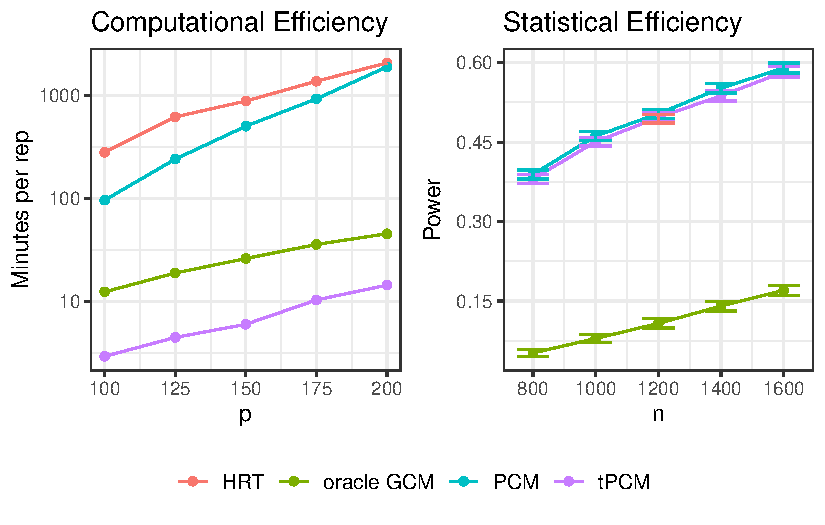
\includegraphics{figures/figure_1.pdf}
		\caption{A comparison of the computational and statistical performance of our method, tPCM, with state-of-the-art competitors. The left panel was from a simulation with larger sample size and number of predictors that focused on computational performance, while the right panel was from a simulation that focused on statistical performance.}
		\label{fig:comp_stat_efficiency}
	\end{figure}
	
	The tPCM satisfies each of the criteria considered in Table~\ref{tab:comparison}, as we verify using both theory and simulations. In particular, we prove that the tPCM is doubly robust, and we observe Type-I error control in our numerical simulations. By its construction, the tPCM is powered against general alternatives, and this fact is echoed by excellent power in our numerical simulations. We conduct an extensive simulation study to demonstrate the power and computational efficiency of our method, comparing it with existing methods. Additionally, we apply the tPCM to a breast cancer dataset to show its practical applicability. The tPCM only requires two machine learning fits and $O(p)$ resamples, making it computationally fast by our definition. As shown in Figure~\ref{fig:comp_stat_efficiency}, it is dramatically faster than both the PCM test and the HRT. Finally, the tPCM produces $p$-values for each variable, by its construction. Code to reproduce these simulations and real data analysis is available at \url{https://github.com/Katsevich-Lab/symcrt2-manuscript/tree/arxiv-v1}.
	
	In addition to our methodological contributions, we provide a novel theoretical insight by showing that the PCM test can be seen as an asymptotic approximation to the HRT. This discovery not only proves the double robustness of the HRT (recall Table~\ref{tab:comparison}) but also establishes a bridge between the model-X and doubly robust strands of literature on conditional independence testing and variable selection.

	\subsection{Related work} \label{sec:related-work}

	Here, we expand on different strands of related work.  
	
	\paragraph{Model-X methods.} There have been several works focusing on Type-I error control for model-X methodologies without requiring the model-X assumption. The Type-I error control of model-X knockoffs when $\law(\prx)$ is estimated in-sample has been studied by \citet{Fan2018a} and \citet{Fan2023}, as discussed above. This question has also been studied when $\law(\prx)$ is estimated out-of-sample \citep{Barber2018, Fan2020}. A conditional variant of model-X knockoffs that allows $\law(\prx)$ to follow a parametric model with unknown parameters was proposed by \citet{Huang2019}. In addition to model-X knockoffs, \citet{CetL16} also proposed the conditional randomization test (CRT) for conditional independence testing, of which the HRT is a special case. The Type-I error of the CRT when $\law(\prx)$ is estimated out-of-sample was studied by \citet{Berrett2019}. A special case of the CRT called the distilled CRT (dCRT; \cite{Liu2020}) was shown to be doubly robust by \citet{Niu2022}. Other variants of the CRT have also been proposed for their improved robustness properties \citep{Berrett2019,Li2022b,Barber2020,Zhu2023}. Other variants of the CRT have also been proposed for improved computational performance, including the HRT and several others \citep{Tansey2018,Zhong2021,Li2021c,Liu2020}. In the latter category, tests either are not suited for producing fine-grained $p$-values for each variable or require $O(p^2)$ resamples to get them. 
 	
	\paragraph{Doubly robust methods.}

	Another related strand of literature focuses on doubly robust testing and estimation. The GCM test \citep{Shah2018} uses a product of residuals statistic to test conditional independence against alternatives where the expected conditional covariance~\eqref{eq:expected-conditional-covariance} is nonzero. Minimax estimation of the expected conditional covariance has also been extensively studied; see for example \citet{Robins2008,Robins2009}. The weighted GCM test \citep{Scheidegger2022a} extends the GCM test for power against broader classes of alternatives. For sensitivity against even more general departures from the null, estimation and testing of functionals related to
	\begin{equation}
	\varphi_j(\law) \equiv \E_{\law}[(\pry - \E_{\law}[\pry \mid \prx_{\minus j}])^2] - \E_{\law}[(\pry - \E_{\law}[\pry \mid \prx])^2]
	\label{eq:nonlinear-r-squared}
	\end{equation}
	have been considered \citep{Zhang2020,Williamson2021,Williamson2021a,Dai2022,Lundborg2022a,Hudson2023,Verdinelli2024}, including the PCM test. The advantage of this functional is that it is equal to zero if and only if conditional independence $H_{0j}$ holds, but its disadvantage is that it is not pathwise differentiable at such points, since they lie on the boundary of the space of values taken on by the functional. Different methods have different approaches to mitigating this issue. However, all of these methods were designed to examine a single variable at a time, so naive application of these approaches to each of the predictor variables is computationally expensive when the number of predictors is large.

	\paragraph{Work at the intersection.}

	In a previous work \citep{Niu2022}, we established an initial bridge between the model-X and doubly-robust literatures by proving the asymptotic equivalence between two conditional independence tests with power against partially linear alternatives: the dCRT \citep{Liu2020} and the GCM test \citep{Shah2018}. In this work, we strengthen this bridge by proving the asymptotic equivalence between the HRT and the PCM test, which have power against more general classes of alternatives.

	\section{Background: The PCM test and the HRT}
%\textcolor{red}{TODO: discuss the strength and weakness of both the methods and motivate the tPCM which has both}

%Narrowing our focus, we shift to testing a single hypothesis in a setting where we have a predictor $\prx \in \R$, response $\pry \in \R$, and a high-dimensional covariate vector $\prz \in \R^{p}$, all drawn from a joint distribution $(\prx, \pry, \prz) \sim \law$—noting that $\law$ may depend on $n$. We aim to test the hypothesis of conditional independence:
%\begin{equation}
%	H_{0n}: \pry \independent \prx\ |\ \prz
%	\label{conditional-independence}
%\end{equation}
%at level $\alpha \in (0,1)$ using $n$ data points 
%\begin{equation}
%	\label{eq:xyz}
%	(\srx, \sry, \srz) \equiv \{(\srx_i, \sry_i, \srz_i)\}_{i = 1, \dots, n} \iidsim \law. 
%\end{equation}

In this section, we define the PCM test and the HRT. In preparation for this, we introduce some notation. Let
\begin{equation}
m(\prx) \equiv \E_\law [\pry \mid \prx] \quad \textnormal{and} \quad m_j(\prx_{\minus j}) \equiv \E_\law [\pry \mid \prx_{\minus j}].
\end{equation}
For a fixed function $\widehat f(\prx)$, we will denote
\begin{equation}
m_{\widehat f}(\prx_{\minus j}) \equiv \E_\law [\widehat f(\prx) \mid \prx_{\minus j}].
\end{equation}
Many of the quantities we introduce will be indexed by $j$, though at times, we omit this index to lighten notation. We do not assume the model-X setting, so we treat $\law(\prx)$ as unknown. Finally, the set of null laws $\law$ for predictor $j$ is explicitly given by
\begin{equation}
	\nulllaws_{n,j} \equiv \{\law: \law(\prx_j, \pry \mid \prx_{\minus j}) = \law(\prx_{j}\mid\prx_{\minus j}) \times \law(\pry\mid\prx_{\minus j})\}.
\end{equation}

\subsection{Projected covariance measure}\label{sec:vPCM}
In this section, we describe a ``vanilla'' version of the PCM methodology proposed in \citet{Lundborg2022a}, which we shall refer to as vPCM. vPCM is a special case of the slightly more involved PCM, which retains its essential ingredients but omits some steps that do not affect the asymptotic statistical performance. Explicitly, we omit steps 1 (iv) and 2 of Algorithm 1 in \citet{Lundborg2022a}. The full algorithm is displayed in Algorithm \ref{alg: pcm}, but we describe it in words now. We begin by splitting our data into $D_1 \cup D_2$, with $D_1$ and $D_2$ containing $n$ and $m$ samples, respectively.  We estimate $\widehat m(\prx) \equiv \widehat{\E}[\pry \mid \prx]$ on $D_2$, and then we regress it onto $\prx_{\minus j}$ using $D_2$ to obtain $\widecheck m_j(\prx_{\minus j})$. We denote the difference of the two quantities $\widehat f_j(\prx) \equiv \widehat m(\prx) - \widecheck m_j(\prx_{\minus j})$. The quantity $\widehat f_j(\prx)$ is then tested for association with $\pry$, conditionally on $\prx_{\minus j}$ on $D_1$. To this end, we regress $\pry$ on $\prx_{\minus j}$ using $D_1$ to obtain an estimate of $\E[\pry|\prx_{\minus j}]$, which we call $ \widetilde{m}_j(\prx_{\minus j})$. We also regress $\widehat f_j(\prx)$ on $\prx_{\minus j}$ using $D_1$ to obtain $\widehat m_{\widehat f_j} (\prx_{\minus j})$.  We define the product of residuals stemming from the two regressions as 
\begin{equation}
L_{ij} \equiv (\sry_i - \widetilde{m}_j(\srx_{i,\minus j}))(\widehat f_j(\srx_i) - \widehat m_{\widehat f_j} (\srx_{i,\minus j})) 
\label{eq:l-i-j}
\end{equation}
and define the vanilla PCM statistic for predictor $j$ as:
\begin{equation}
	T^{\textnormal{vPCM}}_j \equiv \frac{\frac{1}{\sqrt n} \sum_{i=1}^n L_{ij}}{\sqrt{\frac{1}{n} \sum_{i=1}^n L_{ij}^2 - \left(\frac{1}{n} \sum_{i=1}^n L_{ij}\right)^2 }}
\label{eq:vpcm-test-stat}
\end{equation}
Under the null hypothesis, $T_j^{\textnormal{vPCM}}$ is a sum of random quantities and for sufficiently large $n$ and under appropriate conditions, the Central Limit Theorem (CLT) is expected to apply. Hence, we can compare our statistic to the quantiles of the normal distribution and reject for large values.
Our test is defined as
$$
\phi_j^{\textnormal{vPCM}}(\srx,\sry) \equiv \mathbbm{1}\left(T^{\textnormal{vPCM}}_j(\srx,\sry) > z_{1-\alpha}\right).
$$
Aside from the fitting of $\widehat m(\prx)$, the steps are repeated for each predictor $j = 1,\ldots,p$.


\begin{algorithm}[h]
	\SetAlgoLined % This ensures lines are numbered
	\KwIn{Data $\{(\srx_{i}, \sry_i)\}_{i = 1, \dots, m + n}$}
	Split the data into $D_1 \cup D_2$, with $D_1$ and $D_2$ containing $n$ and $m$ samples, resp.
	
	Estimate $\E[\pry \mid \prx]$ on $D_2$, call it $\widehat m(\prx)$.
	
	\For{$j \gets 1$ \KwTo $p$}{
		Regress $\widehat m(\prx)$ on $\prx_{\minus j}$ using $D_2$ to obtain $\widecheck m_j(\prx_{\minus j})$ and define $\widehat f_j(\prx)  \equiv \widehat m(\prx) - \widecheck m_j(\prx_{\minus j})$.

		Using $D_1$, regress $\sry$ on $\prx_{\minus j}$ to obtain an estimate $\widetilde{m}_j(\prx_{\minus j})$ of $\E[\pry|\prx_{\minus j}]$.

		Also on $D_1$, regress $\widehat f_j(\prx)$ on $\prx_{\minus j}$ to obtain $\widehat m_{\widehat f_j} (\prx_{\minus j})$.

		Compute $T^{\textnormal{vPCM}}_j$ based on equations~\eqref{eq:l-i-j} and~\eqref{eq:vpcm-test-stat}.

		Set $p_j \equiv 1 - \Phi(T^{\textnormal{vPCM}}_j)$.
	}
	\Return $\{p_j\}_{j = 1, \dots, p}$.
	
	\caption{Vanilla PCM}
	\label{alg: pcm}
\end{algorithm}

The primary disadvantage of Algorithm \ref{alg: pcm} is that it requires 3$p$+1 machine learning fits, which we would expect to be computationally difficult when $p$ is large. On the other hand, since Algorithm \ref{alg: pcm} uses asymptotic approximation, it does not require any resampling.

\subsection{Holdout Randomization Test} 
In this section, we describe the holdout randomization test (HRT), displayed as Algorithm~\ref{alg: hrt}, which is identical to Algorithm 2 of \citet{Tansey2018} except the estimation of $\law(\prx)$, which the latter authors assumed known. As before, we divide our data into two halves, $D_1$ and $D_2$. On $D_2$, we learn the function $\widehat{m}(\prx) \equiv \widehat{\E}[\pry \mid \prx]$ and the law $\lawhat(\prx)$. On $D_1$, we compute the mean-squared error (MSE) test statistic
\begin{equation}\label{eq:HRT-test}
	T^{\textnormal{HRT}}(\srx, \sry) \equiv \frac{1}{n} \sum_{i=1}^n (\sry_i - \widehat{m}(\srx_i))^2.
\end{equation}
Next, we exploit the fact that under the null hypothesis, the conditional distribution $\law(\prx_j \mid \prx_{\minus j}, \pry)$ is the same as $\law(\prx_j \mid \prx_{\minus j})$, for which we have the estimate $\lawhat(\prx_j|\prx_{\minus j})$. Therefore, we can approximate the distribution of $T^{\textnormal{HRT}}(\srx, \sry)$ conditional on $\sry, \srx_{\minus j},D_2$ by resampling $\widetilde \srx_i \indsim \lawhat(\srx_{i,j}|\srx_{i,\minus j})$ $B_{\textnormal{HRT}}$ times for each $i=1,\ldots,n$. In particular, we can approximate the following conditional quantile:
\begin{equation*}
	C_j(\sry,\srx_{\minus j}) \equiv \Q_{1-\alpha}\left[\frac{1}{n} \sum_{i=1}^n (\sry_i - \widehat m(\widetilde{\srx}_{i,j},\srx_{i,\minus j}))^2 \mid \sry, \srx_{\minus j},D_2\right].
\end{equation*}
The HRT for predictor $j$ is then defined as
\begin{equation*}
\phi_j^{\textnormal{HRT}}(\srx,\sry) \equiv \mathbbm{1}\left(T^{\textnormal{HRT}}(\srx,\sry) \leq C_j(\sry,\srx_{\minus j}) \right).
\end{equation*}
The steps are than repeated for each predictor $j = 1,\ldots,p$. Algorithm~\ref{alg: hrt} describes how to compute the HRT $p$-values for each variable. 

\begin{algorithm}[h]
	\SetAlgoLined % This ensures lines are numbered
	\KwIn{Data $\{(\srx_{i}, \sry_i)\}_{i = 1, \dots, m + n}$, $B_{\textnormal{HRT}}$ resamples.}
	Split the data into $D_1 \cup D_2$, with $D_1$ and $D_2$ containing $n$ and $m$ samples, resp.
	
	Estimate $\E[\pry \mid \prx]$ on $D_2$, call it $\widehat m(\prx)$.

	Estimate $\law(\prx)$ on $D_2$, call it $\lawhat(\prx)$.

	Compute test statistic $T^{\textnormal{HRT}}$ as in equation~\eqref{eq:HRT-test}.
	
	\For{$j \gets 1$ \KwTo $p$}{
		\For{$b \gets 1$ \KwTo $B_{\textnormal{HRT}}$}{
			Sample $\widetilde{\srx}_{i,j} \sim \lawhat(\srx_j \mid \srx_{i, \minus j})$ for all $i \in D_1$.

			Compute $\widetilde T_j^b \equiv \frac{1}{n} \sum_{i=1}^n (\sry_i - \widehat{m}(\widetilde{\srx}_{i,j}, \srx_{i,\minus j}))^2$.
		}

		Set $p_j \equiv \frac{1}{B_{\textnormal{HRT}} + 1} \left(1 + \sum_{b = 1}^{B_{\textnormal{HRT}}} \mathbbm{1}\left[ T^{\textnormal{HRT}} \leq \widetilde T_j^b \right] \right)$.
	}
	\Return $\{p_j\}_{j = 1, \dots, p}$.
	\caption{Holdout Randomization Test}
	\label{alg: hrt}
\end{algorithm}

The primary disadvantage of Algorithm \ref{alg: hrt} is that it requires $p \times B_{\textnormal{HRT}}$ resamples. $B_{\textnormal{HRT}}$ would be required to be large when using the Bonferroni correction to control the family wise error rate, and $p$ is large. On the other hand, an attractive property of Algorithm \ref{alg: hrt} is that it requires only two machine learning fits.

\section{Best of both worlds: Tower PCM}\label{sec:doubly-robust-tower-PCM}

In this section, we introduce the tower PCM method (Section~\ref{sec:tPCM}), followed by a discussion of its computational and statistical properties (Sections~\ref{sec:tpcm-computation} and~\ref{sec:tpcm-type-i-error-control}, respectively).

\subsection{The tower PCM algorithm} \label{sec:tPCM}

The computational bottleneck in the application of the PCM test (Algorithm~\ref{alg: pcm}) is the repeated application of regressions to obtain $\E[\pry \mid \prx_{\minus j}]$ for each $j$. Our key observation is that if we compute estimates $\lawhat(\prx)$ and $\widehat m(\prx) \equiv \widehat{\E}[\pry \mid \prx]$ (as in the first two steps of the HRT), then we can construct estimates of $\E[\pry \mid \prx_{\minus j}]$ for each $j$ without doing any additional regressions. Indeed, note that by the tower property of expectation, we have
\begin{equation*}
\E[\pry \mid \prx_{\minus j}] \equiv \E_{\law}[m(\prx) \mid \prx_{\minus j}] \approx \E_{\law}[\widehat m(\prx) \mid \prx_{\minus j}, D_2] \approx \E_{\lawhat}[\widehat m(\prx) \mid \prx_{\minus j}, D_2] \equiv \widehat m_j(\prx_{\minus j}).
\end{equation*}
To compute the quantity $\widehat m_j$, we can use conditional resampling based on $\lawhat(\prx_j \mid \prx_{\minus j})$. Unlike the HRT, however, the goal of conditional resampling is to compute expectations rather than tail probabilities, and therefore, much fewer conditional resamples are required. Equipped with $\widehat m_j$, we can proceed as in the PCM test by computing products of residuals
\begin{equation}
	R_{ij} \equiv (\sry_i  - \widehat m_j(\srx_{i,\minus j}))(\widehat m(\srx_i) - \widehat{m}_j(\srx_{i,\minus j})),
\end{equation}
and constructing the test statistic	
\begin{align}
	T^{\textnormal{tPCM}}_j \equiv \frac{\frac{1}{\sqrt n} \sum_{i=1}^n R_{ij}}{\sqrt{ \frac{1}{n}\sum_{i=1}^n R_{ij}^2 - \left(\frac{1}{n} \sum_{i=1}^n R_{ij} \right)^2}} \equiv \frac{\frac{1}{\sqrt n} \sum_{i=1}^n R_{ij}}{\widehat \sigma_n},
\end{align}
which we expect is asymptotically normal under the null hypothesis. This yields the test
\begin{equation}
\phi_j^{\textnormal{tPCM}}(\srx,\sry) \equiv \mathbbm{1}\left(T^{\textnormal{tPCM}}_j(\srx,\sry) > z_{1-\alpha}\right).
\end{equation}
These steps lead to Algorithm~\ref{alg: tpcm}.

\begin{algorithm}[h]
	\SetAlgoLined % This ensures lines are numbered
	\KwIn{Data $\{(\srx_{i}, \sry_i)\}_{i = 1, \dots, m + n}$, $B_{\textnormal{tPCM}}$ resamples.}
	Split the data into $D_1 \cup D_2$, with $D_1$ and $D_2$ containing $n$ and $m$ samples, resp.
	
	Estimate $\E[\pry \mid \prx]$ on $D_2$, call it $\widehat m(\prx)$.

	Estimate $\law(\prx)$ on $D_2$, call it $\lawhat(\prx)$.
	
	\For{$j \gets 1$ \KwTo $p$}{
		\For{$k \gets 1$ \KwTo $B_{\textnormal{tPCM}}$}{
			Sample $\widetilde{\srx}_{i,j} \sim \lawhat(\srx_j \mid \srx_{i, \minus j})$ for all $i$.
		}
		
		Compute $\widehat{m}_j (\srx_{i,\minus j}) \equiv \frac{1}{B_{\textnormal{tPCM}}}\sum_{k=1}^{B_{\textnormal{tPCM}}} \widehat{m} (\widetilde{\srx}_{i,j}, \srx_{i,\minus j}) $ for all $i$.

		Define $R_{ij} \equiv (\sry_i  - \widehat{m}_j (\srx_{i,\minus j}))(\widehat m(\srx_i) - \widehat{m}_j (\srx_{i,\minus j}))$ for $i$ in $D_1$.

		Compute $T^{\textnormal{tPCM}}_j \equiv \frac{\frac{1}{\sqrt n} \sum_{i=1}^n R_{ij}}{\sqrt{ \frac{1}{n}\sum_{i=1}^n R_{ij}^2 - \left(\frac{1}{n} \sum_{i=1}^n R_{ij}\right)^2}}$.


		Set $p_j \equiv 1 - \Phi(T^{\textnormal{tPCM}}_j)$.
	}
	\Return $\{p_j\}_{j = 1, \dots, p}$.
	\caption{Tower PCM}
	\label{alg: tpcm}
\end{algorithm}

\subsection{Computational cost comparison} \label{sec:tpcm-computation}
In this subsection, we compare the computational cost of tPCM to that of PCM and HRT. To this end, we consider the following units of computation, which compose the methods considered:

\begin{enumerate}
	\item \texttt{ML(Y|X)}: Training a machine learning model to predict $\sry$ from $\srx$ or $\srx_{\minus j}$
	\item \texttt{ML(X)}: Training a machine learning model to learn the joint distribution of $X$
	\item \verb!ML(X_j|X_-j)!: Training a machine learning model to predict $X_j$ from $X_{\minus j}$
	\item \verb!predict(X_j|X_-j)!: Sampling or predicting from the conditional distribution of $X_j$ given $X_{\minus j}$
	\item \verb!predict(Y|X)!: Predicting $Y$ from $X$ using a trained machine learning model
\end{enumerate}
We can consider each method as having a \textit{learning step} (involving some combination of items 1-3) followed by a \textit{prediction step} (involving some combination of items 4-5). Table~\ref{tab: computational work} summarizes the number of each units of computation required by each method, in terms of the number of variables $p$, the number of resamples for tPCM $B_{\textnormal{tPCM}}$, and the number of resamples for HRT $B_{\textnormal{HRT}}$.

\begin{table}[h!]
	\centering
	\begin{tabular}{|l||c|c|c||c|c|}
		\hline
		& \texttt{ML(Y|X)} & \texttt{ML(X)} & \verb!ML(X_j|X_-j)! & \verb!predict(X_j|X_-j)! & \verb!predict(Y|X)! \\
		\hline
		tPCM & 1 & 1 & 0 & $p \times B_{\textnormal{tPCM}}$ & $p \times B_{\textnormal{tPCM}}$ \\
		PCM & $p$ & 0 & $p$ & $p$ & $p$ \\
		HRT & 1 & 1 & 0 & $p \times B_{\textnormal{HRT}}$ & $p \times B_{\textnormal{HRT}}$ \\
		\hline
	\end{tabular}
	\caption{Computational work required by the methods considered.}
	\label{tab: computational work}
\end{table}

Given Table~\ref{tab: computational work}, tPCM has a substantial computational advantage over PCM under the following mild conditions:
\begin{itemize}
	\item $p \gg 1$ \\ (tPCM has faster machine learning step for $Y|X$)
	\item $p\ \times $ (\verb!ML(Y|X)! + \verb!ML(X_j|X_-j)!) $\gg$ \verb!ML(X)!  \\ (Fitting \verb!ML(X)! for tPCM is negligible compared to repeating ML $p$ times for PCM)
	\item \verb!ML(X_j|X_-j)! + \verb!ML(Y|X)! $ \gg B_{\textnormal{tPCM}} \ \times $ (\verb!predict(X_j|X_-j)! + \verb!predict(Y|X)!) (tPCM's slower prediction step negligible compared to PCM's ML step)
\end{itemize}
On the other hand, tPCM has a substantial computational advantage over HRT under the following mild conditions:
\begin{itemize}
	\item $B_{\textnormal{HRT}} \gg B_{\textnormal{tPCM}}$ \\
	(tPCM has faster prediction step)
	\item $p  \times  B_{\textnormal{HRT}}\ \times$ (\verb!predict(X_j|X_-j)! + \verb!predict(Y|X)!) $ \geq $ \verb!ML(X)! + \verb!ML(Y|X)! \\ (HRT's slower prediction step is a significant proportion of its total computation)
\end{itemize}
In summary, we anticipate that tPCM has a faster machine learning step than PCM and a faster prediction step than HRT. Now that we have established the potential computational advantages of tPCM, we verify its statistical validity.

\subsection{Type-I error control and equivalence to the oracle test} \label{sec:tpcm-type-i-error-control}

In this section, we establish the Type-I error control of the tPCM test. To this end, we will show that the tPCM test is asymptotically equivalent to an oracle test. For the remainder of this section, we will focus on the test of $H_{0j}$ for a single predictor $j$, and sometimes omit the index $j$ to lighten the notation. To define the oracle test, we begin by defining the residuals 
\begin{equation}
\varepsilon_i \equiv \sry_i - m(\srx_{i,\minus j}) \quad \text{and} \quad \xi_i = \widehat{m}(\srx_{i,j},\srx_{i,\minus j}) - \E_{\law} [\widehat{m}(\srx_{i,j},\srx_{i,\minus j}) |\srx_{i,\minus j},D_2],
\end{equation}
Note that $\xi_i$ is defined in terms of the estimated $\widehat m$ rather than the true $m$. The ``oracle'' portion consists of access to the true $\law(\prx)$ to compute the conditional expectation term. Letting 
\begin{equation}
\sigma_n^2 \equiv \mathrm{Var}_\law[\bm{\varepsilon}\bm{\xi} | D_2], 
\end{equation}
the oracle test is defined as
\begin{equation}
\phi_j^{\textnormal{oracle}}(\srx,\sry) \equiv \mathbbm{1}\left(T^{\textnormal{oracle}}_j(\srx,\sry) > z_{1-\alpha}\right), \quad \text{where} \quad T_j^{\textnormal{oracle}} \equiv \frac{1}{\sqrt n \sigma_n} \sum_{i=1}^n\varepsilon_i\xi_i.
\label{eq:oracle-test}
\end{equation}

Next, we define the asymptotic equivalence of two tests $\phi^{(1)}_n, \phi^{(2)}_n: (X,Y) \mapsto [0,1]$ as the statement
$$
\lim_{n\to \infty} \P[\phi_n^{(1)}(X,Y) \neq \phi_n^{(2)}(X,Y)] = 0.
$$
The following set of properties will ensure the equivalence of $\phi_j^{\text{tPCM}}$ and $\phi_{j}^{\text{oracle}}$. The first condition bounds the conditional variance of the error $\varepsilon_i$:
\begin{equation} \label{eq:var-bounded}
	\begin{aligned}
		\exists c_1 > 0, \quad & \P\left[ \max_{i \in [n]}\ \mathrm{Var}_\law(\varepsilon_i | \srx_{i,\minus j},D_2) \leq c_1 \right] \to 1.
	\end{aligned}
\end{equation}
The next condition is written in terms of the conditional chi-square divergence
\begin{equation}
\chi^2(P, Q \mid \mathcal F) \equiv \E_{Q}\left[\left(\frac{dP}{dQ}-1\right)^2\mid \mathcal F\right],
\end{equation}
defined for measures $P$ and $Q$ and a $\sigma$-algebra $\mathcal F$. Using the conditional chi-square divergence to measure the error in the conditional distribution $\law_{\prx_j \mid \prx_{\minus j}}$, we assume this conditional distribution is consistently estimated in the following sense:
\begin{gather}
	\label{eq:uniform-bound-div} \P\left( \max_{i \in [n]}\chi^2\left(\lawhat_{\srx_{i,j}|\srx_{i,\minus j}}, \law_{\srx_{i,j}|\srx_{i,\minus j}} | D_2\right) < c_3\right) \to 1,\\ 
	\label{eq:consistency-of-chi-square-div}	E^2_{\lawhat,n} \equiv \frac{1}{n\sigma_n^2} \sum_{i=1}^n \chi^2\left(\lawhat_{\srx_{i,j}|\srx_{i,\minus j}}, \law_{\srx_{i,j}|\srx_{i,\minus j}} | D_2\right) \E_\law[ \xi_i^2 | \srx_{i,\minus j}, D_2] \overset{p}{\to} 0.
\end{gather}
Similarly, we assume a consistent estimate of $m(\prx) = m_j(\prx_{\minus j})$ (this equality holding because we are under the null):
\begin{equation}\label{eq:consitency-of-reg-func}
	(E'_{\widehat m,n})^2 \equiv \frac{1}{n\sigma_n^2}\sum_{i=1}^n\E_\law[( \widehat m (\srx_{i,j},\srx_{i,\minus j}) - m_j(\srx_{i,\minus j}))^2  \mid D_2,\srx_{i,\minus j}]\E [\xi_i^2|\srx_{i,\minus j},D_2] \overset{p}{\to} 0.
\end{equation}
Also, we define the MSE for $\widehat m$ as follows:
\begin{equation*}
	E^2_{\widehat m,n} = \frac{1}{n\sigma_n^2}\sum_{i=1}^n\E_\law[( \widehat m (\srx_{i,j},\srx_{i,\minus j}) - m_j(\srx_{i,\minus j}))^2  \mid D_2,\srx_{i,\minus j}], 
\end{equation*}
and assume a doubly robust type assumption which states 
\begin{align}\label{eq:doubly-robust-rate}
	E_{\lawhat,n} \cdot E_{\widehat m,n} = o_p(n^{-1/2}).
\end{align}  
Finally, we assume the following Lyapunov-type condition:
\begin{gather}\label{eq:CLT-condition}
	\frac{1}{\sigma_n^{2+\delta}}\E_\law\left[|\bm\varepsilon\bm\xi|^{2+\delta} \mid D_2\right] = o_P(n^{\delta/2}),
\end{gather}
The following theorem establishes the asymptotic validity of our proposed test under the aforementioned assumptions:
\begin{theorem}\label{thm:tower-pcm-type-I-error}
	Given $\law \in \nulllaws_n$ and estimator $\widehat m$ and $\lawhat$ satisfying assumptions~\eqref{eq:var-bounded}, \eqref{eq:uniform-bound-div}, \eqref{eq:consistency-of-chi-square-div}, \eqref{eq:consitency-of-reg-func}, \eqref{eq:doubly-robust-rate} and~\eqref{eq:CLT-condition},
	we have that $\phi_j^{\textnormal{tPCM}}$ is asymptotically equivalent to $\phi_j^{\textnormal{oracle}}$. Additionally, tPCM is asymptotically level $\alpha$:
	$$
	\E_{\law}\left[\phi_j^{\textnormal{tPCM}}(\srx,\sry)\right] \to \alpha.
	$$
\end{theorem}

Next, we provide a simple example in which the assumptions of Theorem~\ref{thm:tower-pcm-type-I-error} are satisfied. 
\paragraph{Linear Model:} For a fixed $p$ we have $(\srx_{i,j},\sry_i,\srx_{i,\minus j}) \in \R \times \R \times \R^p$ for $i=1,\ldots,2n$ i.i.d samples arising out of the linear model:
\begin{align}\label{eq:linear-model}
	\begin{split}
		\sry_i = \beta \srx_{i,j} + \srx_{i,\minus j}^T \gamma + \epsilon_i \\
		\srx_{i,j} = \srx_{i,\minus j}^T\eta + \delta_i, \srx_{i,\minus j}\sim P_{\prx_{\minus j}} 
	\end{split}	
\end{align}
where $\epsilon_i,\delta_i \sim N(0,1)$ and $P_{\prx_{\minus j}}$ has bounded support, i.e. $\exists\, c_{\prx_{\minus j}} >0$ such that $\|\prx_{\minus j}\|_2 \leq c_{\prx_{\minus j}}$. We split our data into two halves and estimate all of the unknown parameters using the least squares estimates; this yields estimates $\widehat m(\prx_j,\prx_{\minus j})$ and $\lawhat_{\prx_j|\prx_{\minus j}}$.
\begin{lemma}\label{lemma:linear-model-type-I-error}
	For the linear model described in \eqref{eq:linear-model}, under the null (i.e. $\beta = 0$), the assumptions \eqref{eq:var-bounded}, \eqref{eq:uniform-bound-div}, \eqref{eq:consistency-of-chi-square-div}, \eqref{eq:consitency-of-reg-func}, \eqref{eq:doubly-robust-rate}, and \eqref{eq:CLT-condition} hold true. Therefore, by Theorem~\ref{thm:tower-pcm-type-I-error} we conclude that $\phi_j^{\textnormal{tPCM}}$ is an asymptotically level $\alpha$ test.
\end{lemma}
At this point, we have established the computational advantages of tPCM as well as its statistical validity. In the next section, we compare the power of tPCM to those of PCM and HRT.

\section{Equivalence of tPCM with existing methods}\label{sec:asym-equiv-tower-PCM}

In this section, we will show that tPCM is asymptotically equivalent to the vPCM (Section~\ref{sec:asymp-equivalence-vPCM-tPCM}) and the HRT (Section~\ref{sec:asymp-equiv-HRT-PCM}).

\subsection{Asymptotic equivalence of vPCM and tPCM} \label{sec:asymp-equivalence-vPCM-tPCM}

To show the equivalence of tPCM and vPCM, we will show that the latter method is equivalent to the oracle test $\phi_j^{\textnormal{oracle}}$ defined in equation~\eqref{eq:oracle-test}, which we have shown is equivalent to tPCM (Theorem~\ref{thm:tower-pcm-type-I-error}). The conditions under which vPCM is equivalent to the oracle test echo those under which \citet{Lundborg2022a} showed that PCM controls type-I error. Define the in-sample MSE for the two regressions $\widetilde m_j$ and $\widehat{m}_{\widehat f_j}$ as follows:
\begin{gather*}
	\mathcal{E}_{\widetilde m} = \frac{1}{n} \sum_{i=1}^n (\widetilde m_j(\srx_{i,\minus j}) - m_j(\srx_{i,\minus j}))^2,\quad
	\mathcal{E}_{\widehat m_{\widehat f}} = \frac{1}{n\sigma_n^2} \sum_{i=1}^n (\widehat m_{\widehat f_j}(\srx_{i,\minus j}) - m_{\widehat f_j}(\srx_{i,\minus j}))^2.
\end{gather*}
We assume the following consistency conditions for the regression functions $\widetilde m_j$ and $\widehat m_{\widehat f_j}$:
\begin{gather}\label{eq:consistency-of-reg-of-Y-on-Z}
	\frac{1}{n\sigma_n^2}\sum_{i=1}^n (\widetilde m_j(\srx_{i,\minus j}) - m_j(\srx_{i,\minus j}))^2 \E[\xi_i^2\mid \srx_{i,\minus j}] \overset{p}{\to} 0.\\
	\label{eq:consistency-of-reg-of-f-hat-on-Z}
	\frac{1}{n\sigma_n^2} \sum_{i=1}^n (\widehat m_{\widehat f_j}(\srx_{i,\minus j}) - m_{\widehat f_j}(\srx_{i,\minus j}))^2\E[\varepsilon^2_i \mid \srx_{i,\minus j}] \overset{p}{\to} 0.
\end{gather} 	
We also assume a doubly robust condition on the product of MSEs:
\begin{equation}\label{eq:doubly-robust-condition-vPCM}
	\mathcal{E}_{\widetilde m} \cdot \mathcal{E}_{\widehat m_{\widehat f}}  = o_p(n^{-1})
\end{equation}

\begin{theorem}\label{thm:equivalence-of-vPCM-oracle}
	Suppose $\law_n \in \nulllaws_n$ is a sequence of laws satisfying~\eqref{eq:CLT-condition}, \eqref{eq:consistency-of-reg-of-Y-on-Z}, \eqref{eq:consistency-of-reg-of-f-hat-on-Z}, and~\eqref{eq:doubly-robust-condition-vPCM}. Then the test $\phi_j^{\textnormal{vPCM}}$ is asymptotically equivalent to the oracle test  $\phi_j^{\textnormal{oracle}}$.
\end{theorem}	

Combining this result with that of Theorem~\ref{thm:tower-pcm-type-I-error}, we obtain the following corollary.

\begin{corollary}
	Let $\law_n \in \nulllaws_n$ be a sequence of laws satisfying~\eqref{eq:var-bounded}, \eqref{eq:uniform-bound-div}, \eqref{eq:consistency-of-chi-square-div}, \eqref{eq:consitency-of-reg-func}, \eqref{eq:doubly-robust-rate}, \eqref{eq:CLT-condition}, \eqref{eq:consistency-of-reg-of-Y-on-Z}, \eqref{eq:consistency-of-reg-of-f-hat-on-Z}, and \eqref{eq:doubly-robust-condition-vPCM}. For any sequence $\law_n'$ of alternative distributions contiguous to the sequence $\law_n$, we have that $\phi_n^{\textnormal{vPCM}}$ is equivalent to $\phi_n^{\textnormal{tPCM}}$ against $\law_n'$ i.e.
	$$
	\lim _{n \rightarrow \infty} \mathbb{P}_{\law_n'}\left[\phi_j^{\textnormal{vPCM}}(\srx, \sry)=\phi_j^{\textnormal{tPCM}}(\srx, \sry)\right]=1 .
	$$
	In particular, these two tests have the same limiting power:
	$$
	\lim _{n \rightarrow \infty} \left\{\mathbb{E}_{\law_n'}\left[\phi_j^{\textnormal{vPCM}}(\srx, \sry)\right] - \mathbb{E}_{\law_n'}\left[\phi_j^{\textnormal{tPCM}}(\srx, \sry)\right]\right\} = 0.
	$$
\end{corollary} 	

Despite equivalence of vPCM and tPCM, we highlight an important distinction between these two methods. tPCM exclusively employs out-of-sample regressions, where the regressions are conducted on a different dataset from which the test statistic is evaluated. In contrast, vPCM utilizes both in-sample and out-of-sample regressions. As was pointed out by \citet{Lundborg2022a}, relying on in-sample regressions can be advantageous in finite samples. Nevertheless, the effects of this distinction vanish asymptotically. 

\subsection{Asymptotic equivalence of HRT and tPCM}\label{sec:asymp-equiv-HRT-PCM}
In this section, we establish the asymptotic equivalence between the HRT and tPCM. This is more complicated than establishing the equivalence between vPCM and tPCM, as the HRT is based on resampling rather than an asymptotic approximation, and its test statistic is less closely related to the PCM test statistic. We proceed in three steps. In the first step, we establish a connection between the HRT and tPCM test statistics (Section~\ref{sec:connecting-HRT-PCM}). In the second step, we show that the difference between the tPCM test statistic and a rescaled variant of the HRT test statistic is asymptotically negligible (Section~\ref{sec:asymptotically-negligible-difference}). In the third step, we show that the HRT cutoff converges to the standard normal cutoff (Section~\ref{sec:convergence-of-rHRT-cutoff}). This leads us to conclude that the HRT and tPCM are asymptotically equivalent (Section~\ref{sec:asymptotic-equivalence-HRT-tPCM}).

\subsubsection{Connecting the HRT and tPCM test statistics} \label{sec:connecting-HRT-PCM}

Let us center and scale $T_j^{\text{HRT}}$ so that a limiting distribution can be obtained, and so that the connection with the tPCM test statistic is clearer. Letting
\begin{equation}
\widehat \xi_i \equiv \widehat m(\srx_i) - \widehat m_j(\srx_{i, \minus j}) \quad \text{and} \quad \widetilde \xi_i \equiv \widehat m(\widetilde \srx_i) - \widehat m_j(\srx_{i, \minus j}),
\end{equation}
we find that 
\begin{equation}
\begin{split}
T_j^{\text{HRT}} &\equiv \frac{1}{n}\sum_{i = 1}^n (\sry_i - \widehat m(\srx_i))^2 \\
&= \frac{1}{n}\sum_{i = 1}^n ((\sry_i - \widehat m_j(\srx_{i, \minus j})) + (\widehat m_j(\srx_{i, \minus j}) - \widehat m(\srx_i)))^2 \\
&= -\frac{2\widehat \sigma_n}{\sqrt{n}} T_j^{\text{tPCM}} + \frac{1}{n}\sum_{i = 1}^n (\widehat m_j(\srx_{i, \minus j}) - \widehat m(\srx_i))^2 + \frac{1}{n}\sum_{i = 1}^n (\sry_i - \widehat m_j(\srx_{i, \minus j}))^2 \\
&\equiv -\frac{2\widehat \sigma_n}{\sqrt{n}} T_j^{\text{tPCM}} + \frac{1}{n}\sum_{i = 1}^n \widehat \sxi_i^2 + \frac{1}{n}\sum_{i = 1}^n (\sry_i - \widehat m_j(\srx_{i, \minus j}))^2.
\end{split}
\end{equation}
Separating the portion depending on $\srx_j$ from the rest, we find that
\begin{equation}
\begin{split}
T_j^{\text{HRT}}&= -\frac{2\sigma_n}{\sqrt{n}}\left(\frac{\widehat \sigma_n}{ \sigma_n} T^{\textnormal{tPCM}}_j (\srx,\sry)  - \frac{1}{2\sqrt n \sigma_n}\sum_{i=1}^n(\widehat \xi_i^2 - \E[\widetilde \xi_i^2 \mid \srx_{i,\minus j},  D_2])\right) \\
&\quad \quad + \frac{1}{n}\sum_{i = 1}^n \E[\widetilde \xi_i^2 \mid \srx_{i,\minus j},  D_2] + \frac{1}{n}\sum_{i = 1}^n (\sry_i - \widehat m_j(\srx_{i, \minus j}))^2 \\
&\equiv -\frac{2\sigma_n}{\sqrt{n}} T^{\textnormal{rHRT}}_j + g(\sry, \srx_{\minus j}, D_2).
\label{eq:hrt-tpcm-relationship}
\end{split}
\end{equation}
We have expressed $T_j^{\text{HRT}}$ as a linear function of a rescaled statistic $T^{\textnormal{rHRT}}_j$, which in turn is a linear function of the tPCM statistic $T^{\textnormal{tPCM}}_j$. Let us define the conditional randomization test based on the re-scaled HRT statistic:
\begin{equation}
\phi_j^{\text{rHRT}}(\srx,\sry) \equiv \mathbbm{1}\left(T^{\text{rHRT}}_j(\srx,\sry) > C'_n(\sry,\srx_{\minus j}) \right),
\end{equation}
where
\begin{equation}
C'_n(\sry, \srx_{\minus j}) \equiv \Q_{1-\alpha}\left[T^{\text{rHRT}}_j(\widetilde \srx_j, \srx_{\minus j},\sry) \mid \sry, \srx_{\minus j}, D_2\right].
\end{equation}
and the resamples $\widetilde \srx_j$ are generated as in step 7 of the HRT (Algorithm~\ref{alg: hrt}). The relationship between $T_j^{\text{HRT}}$ and $T_j^{\text{rHRT}}$~\eqref{eq:hrt-tpcm-relationship} implies that the HRT and rHRT are the same test. Indeed, adding and multiplication by factors not involving $\srx_j$ will be absorbed by the corresponding transformations of the resampling distributions, leaving the test unchanged. We record this fact in the following lemma. 

\begin{lemma}\label{lemma:first-reduction-of-HRT}
	
We have $\phi_j^{\textnormal{HRT}}(\srx,\sry) =\phi_j^{\textnormal{rHRT}}(\srx,\sry)$.
	
\end{lemma}

\subsubsection{Bounding the difference between rHRT and tPCM test statistics} \label{sec:asymptotically-negligible-difference}

Recall from equation~\eqref{eq:hrt-tpcm-relationship} that
\begin{equation}
T_j^{\text{rHRT}}(\srx, \sry) \equiv \frac{\widehat \sigma_n}{ \sigma_n} T^{\textnormal{tPCM}}_j (\srx,\sry)  - \frac{1}{2\sqrt n \sigma_n}\sum_{i=1}^n(\widehat \xi_i^2 - \E[\widetilde \xi_i^2 \mid \srx_{i,\minus j},  D_2]).
\end{equation}
We will provide conditions under which the multiplicative factor $\frac{\widehat \sigma_n}{\sigma_n}$ tends to one, and the additive term $\frac{1}{2\sqrt n \sigma_n}\sum_{i=1}^n(\widehat \xi_i^2 - \E[\widetilde \xi_i^2 \mid \srx_{i,\minus j},  D_2])$ tends to zero. This will imply that the test statistics $T_j^{\text{rHRT}}$ and $T_j^{\text{tPCM}}$ are asymptotically equivalent. The multiplicative factor $\frac{\widehat \sigma_n}{\sigma_n}$ tends to one under the assumptions of Theorem~\ref{thm:tower-pcm-type-I-error}:
\begin{lemma} \label{lem:sigma-hat-n-convergence}
Under the assumptions of Theorem~\ref{thm:tower-pcm-type-I-error}, we have that $\frac{\widehat \sigma_n}{\sigma_n} \convp 1$.
\end{lemma}
\noindent To show that the additive term tends to zero, we require a few more assumptions:
\begin{gather}
	\label{eq:variance-of-m-hat-given-Z}
	\frac{1}{\sigma_n^2} \E\left[ \V\left(\bm{\widehat \xi}^2 \mid \prx_{\minus j}, D_2\right)\mid D_2\right] = o_p(1).\\
	\label{eq:tower-regression-rate-assumption}
	\frac{1}{\sqrt n\sigma_n}\sum_{i=1}^n (\widehat m_j(\srx_{i,\minus j}) - \E\left[\widehat m(\srx_{i,j},\srx_{i,\minus j}) \mid \srx_{i,\minus j}, D_2\right])^2 \overset{p}{\to} 0.\\
	\label{eq:variance-of-xi-rate-assumption}
	\frac{1}{\sqrt n \sigma_n} \sum_{i=1}^n\left(\V_{\lawhat}[\sxi_i \mid \srx_{i,\minus j}, D_2] - \V_{\law}[\sxi_i \mid \srx_{i,\minus j}, D_2]\right)\overset{p}{\to} 0.
\end{gather}
Conditions~\eqref{eq:tower-regression-rate-assumption} and~\eqref{eq:variance-of-xi-rate-assumption} can be seen as rate assumptions on the convergence of $\lawhat$ to $\law$. The former equation quantifies the rate of convergence of $\E_{\lawhat}\left[\widehat m(\prx_j,\prx_{\minus j}) \mid \prx_{\minus j}, D_2\right]$ to $\E_{\law}\left[\widehat m(\prx_j,\prx_{\minus j}) \mid \prx_{\minus j}, D_2\right]$ and the latter of $\V_{\lawhat}[\pxi \mid \prx_{\minus j}, D_2]$ to   $\V_{\law}[\pxi\mid \prx_{\minus j}, D_2]$.
\begin{lemma}\label{lemma:extra-term-in-HRT-vanishes}
Under assumptions~\eqref{eq:variance-of-m-hat-given-Z},~\eqref{eq:tower-regression-rate-assumption} and~\eqref{eq:variance-of-xi-rate-assumption}, we have
\begin{equation}\label{eq:def-E_n}
\frac{1}{\sqrt n \sigma_n}\sum_{i=1}^n(\widehat \xi_i^2 - \E[\widetilde \xi_i^2 \mid \srx_{i,\minus j},  D_2]) \convp 0.
\end{equation}
\end{lemma}
Now that we have connected the rHRT and tPCM test statistics, we proceed to connect their cutoff values.

\subsubsection{Convergence of the rHRT cutoff} \label{sec:convergence-of-rHRT-cutoff}

Here, we provide conditions under which the rHRT cutoff $C'_n(\sry,\srx_{\minus j})$ converges to the standard normal cutoff $z_{1-\alpha}$. We assume the following consistency conditions:
\begin{gather}
	\label{eq:regression-of-Y-on-Z-is-consistent-wrt-L-hat} \frac{1}{n \sigma^2_n} \sum_{i=1}^n(\widehat m_j(\srx_{i,\minus j})-m_j(\srx_{i,\minus j}))^2 \E( \widetilde\sxi^2_i \mid \srx_{i,\minus j},D_2)  \overset{p}{\to} 0.\\
	\label{eq:variance-consistency-condition}
	\frac{1}{n\sigma_n^2} \sum_{i=1}^n \left(\V_{\lawhat}[\sxi_i \mid \srx_{i,\minus j}, D_2] - \V_{\law}[\sxi_i \mid \srx_{i,\minus j}, D_2] \right)\E(\seps_i^2 \mid \srx_{i,\minus j}) \overset{p}{\to} 0.\\
	\label{eq:variance-of-xi-hat-goes-to-zero}\frac{1}{{\sigma_n^2}}\E\left[\V(\widetilde{\pxi}^2 \mid \prx_{\minus j}, D_2)\mid D_2\right] \overset{p}{\to} 0.
	%\label{eq:oracle-test-does-not-accumulate}
	%   \frac{1}{\sqrt n \sigma_n} \sum_{i=1}^n \seps_i\sxi_i \quad \textnormal{does not accumulate near } z_{1-\alpha}
\end{gather}
The first condition can be interpreted as a consistency condition for $\widehat m_j$, while the second condition pertains to variance consistency. Additionally, we assume the following moment condition, which is similar to condition~\eqref{eq:CLT-condition}:
\begin{gather}
	\label{eq:moment-condition-on-product-of-residuals-hat} 
	\frac{1}{\sigma_n^{2+\delta}}\E( |\peps\widetilde{\pxi}|^{2+\delta} \mid D_2) = o_p(n^\delta).
\end{gather}

\begin{lemma}\label{thm:conditional-convergence-of-HRT-to-normality}
	Under assumptions~\eqref{eq:CLT-condition}, \eqref{eq:regression-of-Y-on-Z-is-consistent-wrt-L-hat}, \eqref{eq:variance-consistency-condition}, \eqref{eq:variance-of-xi-hat-goes-to-zero}, and~\eqref{eq:moment-condition-on-product-of-residuals-hat}, we have
	$$
	C'_n(\sry,\srx_{\minus j}) \overset{p}{\to} z_{1-\alpha}.
	$$
\end{lemma}

At this stage, we can put all of the pieces together to show the asymptotic equivalence of the HRT and tPCM.

\subsubsection{Asymptotic equivalence of HRT and tPCM} \label{sec:asymptotic-equivalence-HRT-tPCM}

The following theorem can be deduced from Lemmas~\ref{lemma:first-reduction-of-HRT}, \ref{lem:sigma-hat-n-convergence}, \ref{lemma:extra-term-in-HRT-vanishes}, and~\ref{thm:conditional-convergence-of-HRT-to-normality}.

\begin{theorem}\label{thm:HRT-PCM-equivalence} Suppose $\law_n \in \nulllaws_n$ is a sequence of laws satisfying the assumptions of Theorem~\ref{thm:tower-pcm-type-I-error}, as well as conditions \eqref{eq:variance-of-m-hat-given-Z}, \eqref{eq:tower-regression-rate-assumption}, \eqref{eq:variance-of-xi-rate-assumption}, \eqref{eq:regression-of-Y-on-Z-is-consistent-wrt-L-hat}, \eqref{eq:variance-consistency-condition},~\eqref{eq:variance-of-xi-hat-goes-to-zero}, \eqref{eq:moment-condition-on-product-of-residuals-hat}. Then, the HRT test is equivalent to the tPCM  test against $\law_n$.
\end{theorem}

\noindent One consequence of this theorem is the Type-I error control of the HRT beyond the model-X assumption. 

\begin{corollary}
For a sequence of null laws $\law_n \in \nulllaws_n$ satisfying the assumptions of Theorem~\ref{thm:HRT-PCM-equivalence}, the HRT is asymptotically level $\alpha$.
\end{corollary}

\noindent Another consequence of Theorem~\ref{thm:HRT-PCM-equivalence} is that HRT and tPCM are equivalent under contiguous alternatives, and therefore have equal asymptotic power against contiguous alternatives. 

\begin{corollary}
	If $\law_n'$ is a sequence of alternative distributions contiguous to a sequence \( \law_n \) in \( \nulllaws_n \) satisfying the assumptions of Theorem \ref{thm:HRT-PCM-equivalence}, then the HRT and tPCM tests are asymptotically equivalent against \( \law_n' \). Furthermore, they have equal asymptotic power against $\law_n'$:
\begin{equation}
\lim _{n \rightarrow \infty}\left\{\E_{\law_n'}[\phi_j^{\textnormal{HRT}}(\srx, \sry)] - \E[\phi_j^{\textnormal{tPCM}}(\srx, \sry)]\right\} = 0.
\end{equation}
\end{corollary}

\noindent Finally, we claim that the assumptions of Theorem~\ref{thm:HRT-PCM-equivalence} are satisfied in the linear model~\eqref{eq:linear-model}.
\begin{lemma}\label{lemma:linear-model-equivalence-to-HRT}
	For the linear model described in \eqref{eq:linear-model} with $\beta = 0$, the assumptions of Theorem \ref{thm:HRT-PCM-equivalence} are satisfied, which implies that $\phi_j^{\textnormal{tPCM}}$ is an asymptotically equivalent to $\phi_j^{\textnormal{HRT}}$.
\end{lemma}

By constructing a null distribution through resampling, the HRT accommodates arbitrarily complex machine learning methods for constructing test statistics, whose asymptotic distributions may not be known. However, we find that after appropriate scaling and centering, the resampling-based null distribution essentially replicates the asymptotic normal distribution utilized by the PCM test. Therefore, when testing a single hypothesis in large samples, the additional computational burden of resampling is unnecessary, as the equivalent PCM test can be applied instead. When dealing with a large number of samples and multiple hypotheses, the tPCM test becomes the natural candidate, combining the best aspects of the existing methodologies. For a small number of samples, the HRT remains an attractive option, as it does not rely on asymptotic normality.

	\section{Finite-sample assessment}\label{sec:sim-study}
	In this section, we investigate the finite-sample performance of tPCM with a simulation-based assessment of Type-I error,
	power, and computation time. The Type-I error of choice was the family-wise error rate at level $\alpha = 0.05$. We consider a generalized additive model (GAM) specification for the distribution of $Y \mid X$. The goal of the simulation is to corroborate the findings of the previous sections: (1) tPCM is computationally efficient, (2) tPCM controls the Type-I error, and (3) tPCM is as powerful as HRT and PCM. 
	\subsection{Data-generating model}

	We pick $s$ of the $p$ variables to be nonnull at random. Let $\mathcal{S}$ denote the set of nonnulls. We then define our data-generating model as follows:
	\begin{equation*}
	\law_n(\mathbf{X}) = N(0,\Sigma(\rho)), \ \law_n(\mathbf{Y} \mid \mathbf{X}) = N\left(\sum_{i \in \mathcal{S}, \textnormal{odd}} (X_i - 0.3)^2 / \sqrt{2} \theta + \sum_{i \in \mathcal{S}, \textnormal{even}} - \cos(X_i)\theta,1 \right)
	\end{equation*}
	Here, the covariance matrix $\Sigma(\rho)$ is an AR(1) matrix with parameter $\rho$; that is, $\Sigma(\rho)_{ij} = \rho^{|i-j|}$. Therefore, the entire data-generating process is parameterized by the five parameters $(n, p, s, \rho, \theta)$; see Table \ref{tab:gam sim parameters}. We vary each of the five parameters across five values each, setting the remaining to the default values (in bold).

	\begin{table}[h!]
		\centering
		\begin{tabular}{ccccc}
			\hline
			$n$ & $p$ & $s$ & $\rho$ & $\theta$ \\
			\hline
			800 & 30 & 4 & 0.2 & 0.15 \\
			1000 & 40 & 8 & 0.35 & 0.2 \\
			\textbf{1200} & \textbf{50} & \textbf{12} & \textbf{0.5} & \textbf{0.25} \\
			1400 & 60 & 16 & 0.65 & 0.3 \\
			1600 & 70 & 20 & 0.8 & 0.35 \\
			\hline
		\end{tabular}
		\caption{The values of the sample size $n$, covariate dimension $p$, sparsity $s$, autocorrelation of covariates $\rho$, and signal strength $\theta$ used for the
		simulation study. Each of the parameters $n$, $p$, $s$, $\rho$, $\theta$ was varied among the values displayed in the
		table while keeping the other four at their default values, indicated in bold. For example, $p = 50$, $s = 12$, $\rho = 0.5$, $\theta = 0.25$ were kept fixed while varying $n \in \{800, 1000, 1200, 1400, 1600\}$.}
		\label{tab:gam sim parameters}
	\end{table}

	\subsection{Methodologies compared}

	%We applied each of the four methods below, in conjunction with a Bonferroni correction at level $\alpha = 0.05$ to control the family-wise error rate.
	We applied the four methods tPCM, HRT, PCM, and oracle GCM in conjunction with a Bonferroni correction at level $\alpha = 0.05$ to control the family-wise error rate. The PCM implementation was more or less true to Algorithm 1 of \citet{Lundborg2022a}. For all methods, quantities such as $\E[\pry \mid \prx]$ and $\E[f_j(\prx_j) \mid \prx_{-j}]$ were fit using (sparse) GAMs. tPCM and HRT exploited knowledge of the banded structure and so $\law(\prx)$ was fit using a banded precision matrix estimate. PCM was also endowed with knowledge of the banded covariance structure. This meant that for any step requiring a $\E[f_j(\prx_j) \mid \prx_{-j}]$ fit, we actually only regressed $f_j(\prx_j)$ on $\prx_{j-1}$ and $\prx_{j+1}$, since $\prx_j$ is independent of all other $\mathbf{X}_k$ given $\prx_{j-1}$ and $\prx_{j+1}$. Oracle GCM was given knowledge of the true $\E[\pry \mid \prx]$ and $\law(\prx)$ models. We defer the remaining details of the method implementations to Appendix~\ref{sec:simulation-study-details}. 
	
	%Next, we also display in Table \ref{tab:method comparison} a comparison of the compared methodologies in terms of nuisance fits and construction of the null distribution. Consider the situation where the computation time of learning $\law(\mathbf{X})$, $\mathbb{E}[\mathbf{X}_j \mid \mathbf{X}_{\minus j}]$, $\mathbb{E}[\mathbf{Y} \mid \mathbf{X}]$, and $\mathbb{E}[\mathbf{Y} \mid \mathbf{X}_{\minus j}]$ are of the same order. Then for learning of the nuisances, PCM is by far the slowest, as it requires $2p + 1$ fits whereas the others only require $2$. Meanwhile, in the scenario where Bonferroni is used to control the family-wise error rate, HRT, being a resampling-based method, would require a minimum of $p / \alpha$ resamples for each variable to have any power. When $p = 50$ and $\alpha = 0.05$, this minimum threshold is 1000 resamples. Meanwhile, the tower methods require much fewer resamples, as the purpose of the resampling for the tower methods is to obtain a good fit for a conditional mean of some complicated function. All methods used Bonferroni as the multiplicity correction.

	\begin{remark}
	Here we justify the omission of three additional methods from our simulation study. First, we omit the holdout grid test (HGT), a faster version of HRT proposed by \citet{Tansey2018}. The HGT employs a discrete, finite grid approximation and a caching strategy. \citet{Tansey2018} theoretically demonstrated the validity of the procedure under the model-X assumption. We chose to omit this method because when the joint distribution of $\prx$ is not known but estimated, the method may no longer be valid and/or depends on the level of discretization chosen. Furthermore, this method trades off computational resources for memory resources, complicating the comparison. Second, we omit a method proposed by \citet{Williamson2021a} for testing whether the functional~\eqref{eq:nonlinear-r-squared} equals zero because simulations in \citet{Lundborg2022a} demonstrated a sizable gap in power when compared with PCM. Finally, we omitted model-X knockoffs since we desired family-wise error rate control, and model-X knockoffs is not designed to produce fine-grained $p$-values necessary to control this error rate.
	\end{remark}

	% \begin{table}
	% 	\centering
	% 	\begin{tabular}{l|cccc}
	% 		\hline
	% 		\textbf{Learned quantities} & \textbf{oracle GCM} & \textbf{HRT} & \textbf{PCM} & \textbf{tPCM} \\
	% 		\hline
	% 		$\law(\mathbf{X})$ & \checkmark & \checkmark & \textsf{X} & \checkmark \\

	% 		$\mathbb{E}[\mathbf{X}_j \mid \mathbf{X}_{\minus j}]$ for all $j$ & \textsf{X} & \textsf{X} & \checkmark & \textsf{X} \\

	% 		$\mathbb{E}[\mathbf{Y} \mid \mathbf{X}]$ & \checkmark & \checkmark & \checkmark & \checkmark  \\
	
	% 		$\mathbb{E}[\mathbf{Y} \mid \mathbf{X}_{\minus j}]$ for all $j$ & \textsf{X} & \textsf{X} & \checkmark & \textsf{X} \\
	% 		\hline
	% 		\textbf{Null distribution}& & & &  \\
	% 		\hline
	% 		Conditional resampling & \textsf{X} & \checkmark & \textsf{X} & \textsf{X} \\
	% 		Asymptotic $N(0,1)$ & \textsf{X} & \textsf{X} & \checkmark & \textsf{X}  \\
	% 		Hybrid & \checkmark & \textsf{X} & \textsf{X} & \checkmark \\
	% 		\hline
	% 	  \end{tabular}
	% 	  \caption{A comparison of the properties of the methods evaluted in the simulation study.}
	% 	\label{tab:method comparison}
	% \end{table}

	\subsection{Simulation results}

	Results for power and computation time are presented in Figures \ref{fig:power} and \ref{fig:computation} respectively. Figure \ref{fig:fwer} in Appendix~\ref{sec:fwer} displays the family-wise error of the methods. Below are our observations from these results:

	\begin{itemize}
		\item As we expect, all methods tend in improve in terms of power as $n$ increases, amplitude increases, $p$ decreases, and $\rho$ decreases. For $s$, there no such monotonic relationship.
		\item All methods control the family-wise error rate, indicating that in this setting, the $\law(\pry\mid \prx)$ and $\law(\prx)$ are learned sufficiently well.
		\item The oracle GCM has significantly lower power than the other methods, as the test statistic it is based on is most powerful against partially linear alternatives, which is not the case in the simulation design. The other methods have roughly equal power.
		\item Among the three powerful methods, tPCM is by far the fastest, with the gap widening considerably as $p$ grows. 
 	\end{itemize}

	\begin{figure}[H]
		\centering
		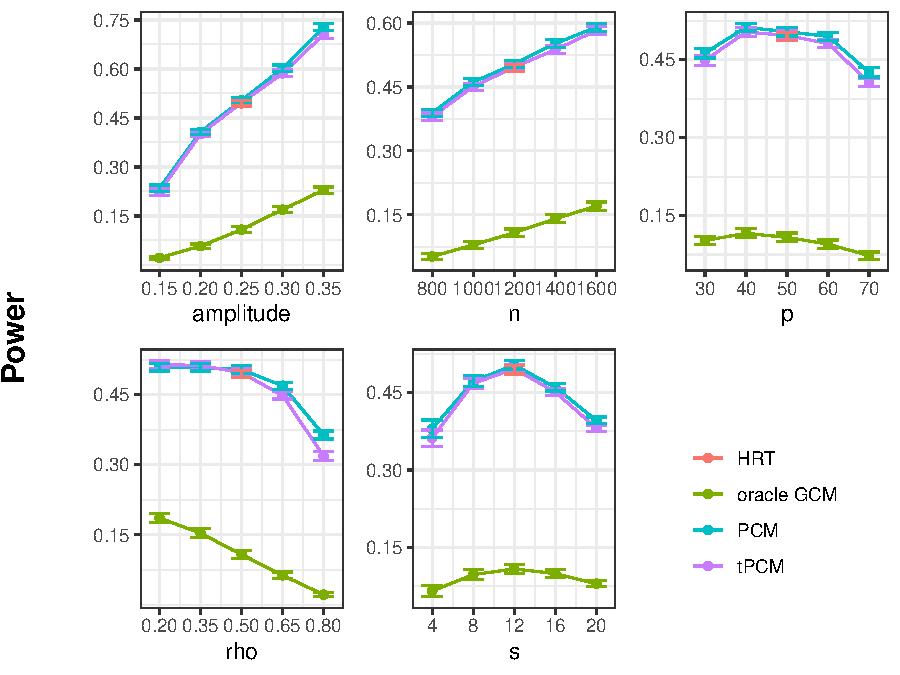
\includegraphics{figures/power_stat.pdf}
		\caption{Power: in each plot, we vary one parameter. Each point is the average of 400 Monte Carlo replicates, and the error bars are the average $\pm 2 \times \widehat{\sigma}_p$, where $\widehat{\sigma}_p$ is the Monte Carlo standard deviation divided by $\sqrt{400}$.}
		\label{fig:power}
	\end{figure}
	\begin{figure}[H]
		\centering
		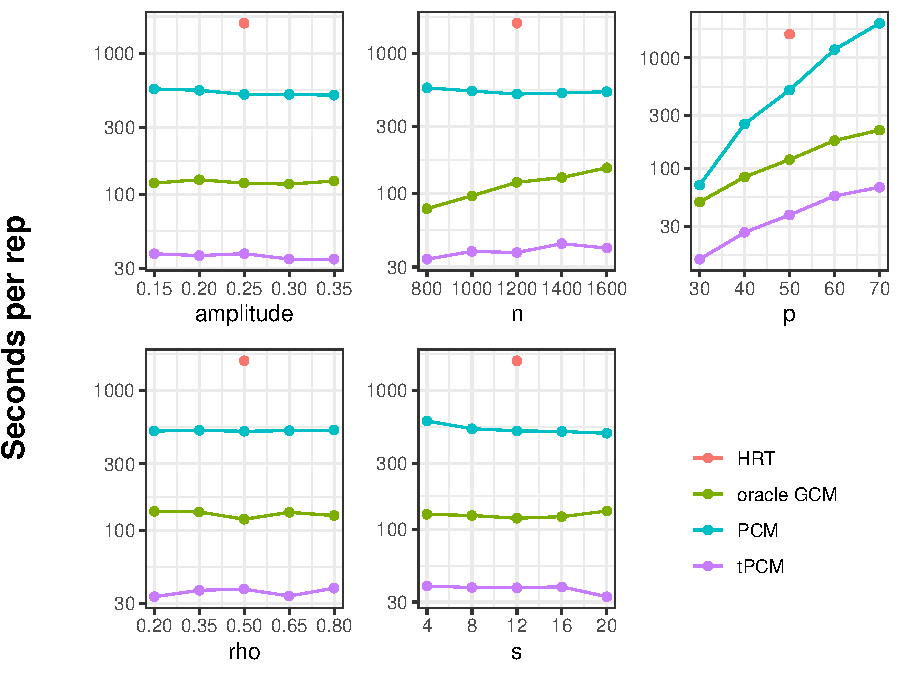
\includegraphics{figures/computation_stat.pdf}
		\caption{Computation: in each plot, we vary one parameter. Each point is the average of 400 Monte Carlo replicates.}
		\label{fig:computation}
	\end{figure}

	\subsection{Computational comparison in a larger setting}
	In the main simulation setting, we chose smaller $n$ and $p$ so that it would be computationally feasible to run 400 Monte Carlo replicates of all methods to assess statistical performance. To further demonstrate the computational advantage of tPCM, we considered a larger setting with the same data-generating model as before, but with different parameters. Specifically, we fixed $n = 2500$, $p = 100$, $\rho = 0.5$, $\theta = 0.25$, $s = 15$, and varied $p \in \{100, 125, 150, 175, 200\}$.  We forego any statistical comparison and simply measure the time taken to perform each procedure once for each of the five settings of $p$. HRT, PCM, and tPCM all used a 0.4 training proportion, HRT used $5 \times p / 0.05$ resamples, and tPCM and oracle GCM used 25 resamples. These results were already shown in the left panel of Figure \ref{fig:comp_stat_efficiency} in Section~\ref{sec:our-contributions}. As expected, the computational gap between tPCM and HRT and PCM widens as $p$ increases, and when $p = 200$, tPCM is more than 130 times faster than HRT and PCM.

\section{Application to breast cancer dataset}
\subsection{Overview of the data}
As a final illustration of our method, we apply tPCM to a breast cancer dataset from \citet{Curtis2012}, which has been previously analyzed in the statistical literature by \citet{Liu2020} and \citet{Li2021c}. The data consist of $n = 1396$ positive cases of breast cancer categorized by stage (the outcome variable) and $p = 164$ genes, for which the expression level (mRNA) and copy number aberration
(CNA) are measured. We seek to discover genes that are associated with stage of breast cancer, conditional on the remaining genes. Statistically, we set the family-wise error rate to be $\alpha = 0.1$. The data is preprocessed using the same steps as in \citet{Liu2020}; we refer the reader to Appendix E of \citet{Liu2020} for more details. The stage of cancer outcome is binary, and the gene expression predictors are continuous.

\subsection{Methods and their implementations}
%As in the simulation study, we applied four methods to the data, which were HRT, tPCM, PCM, and tower GCM (tGCM). The methods are similar to those from the simulations, but we describe the implementations for each method and their specific hyperparameters. We also describe the tGCM procedure, which is similar to the oracle GCM procedure from the simulation.

As in the simulation study, we applied four methods to the data, which were HRT, tPCM, PCM, and tower GCM (tGCM). The methods are similar to those from the simulations, and we again fit $\E[\pry \mid \prx]$ and $\E[f_j(\prx_j) \mid \prx_{\minus j}]$ using a sparse GAM. One major distinction, however, was that the covariance structure was not banded as in the simulation, so we fit $\mathcal{L}(\prx)$ using the graphical lasso. This also had implications for the $\E[f_j(\prx_j) \mid \prx_{\minus j}]$ fits in PCM. We leave the details of the implementations for each method and their specific hyperparameters to Appendix~\ref{sec:data-analysis-details}, as well as an explanation of the tGCM procedure, which is similar to the oracle GCM procedure from the simulation.

\begin{remark}
Even though the outcome was binary, we chose to fit $\E[\pry \mid \prx]$ and $\E[\pry \mid \prx_{\minus j}]$ using a gaussian family GAM. This choice has precedent (\citet{Liu2020} used a non-logistic statistic when implementing the resampling-free version of dCRT), but was also motivated by computational concerns, as a fit for $\E[\pry \mid \prx]$ with a GAM with a logit link took 5-6 times as long. Given that PCM took a bit more than 1.5 days to run with the Gaussian link, we estimate that it would have taken over a week to run, which exceeds the maximum run time allowed on our cluster. 
\end{remark}

\subsection{Results}
We now report the identities of the rejected genes produced by the four methods at level $\alpha = 0.1$ using the Bonferroni correction, as well as the computation time in minutes. These are summarized in Table \ref{tab:real_da_results}. Notably, tower PCM returns the most rejections with 4, followed by HRT and tower GCM with 3, and none from PCM. In addition, tower PCM performs the best computationally, taking just over 8 minutes due to only estimating two nuisances and using 25 resamples for each predictor. HRT likewise estimated two nuisances, but was slower due to applying a black-box function to 5000 resamples. tGCM was bit a slower than tPCM, since it fit two nuisances 5 times corresponding to each fold on 80\% of the data. PCM was by far the slowest since it had to fit regressions $\E[\pry \mid \prx_{\minus j}]$ and $\E[f_j(\prx_j) \mid \prx_{\minus j}]$ $p$ times each, and such steps were more costly than resampling. As for the discovered genes, tPCM had the most rejections with 4, 3 of which were also rejected by HRT. This gives further evidence to the theoretical claim of asymptotic equivalence between HRT and tPCM. It is possible that if we had used more resamples for HRT, it would have discovered the fourth gene that tPCM did, though of course at a greater computational cost. Given our theoretical result regarding equivalence between tPCM and vPCM, it was surprising to see PCM make no rejections. One potential explanation is that there is a disconnect between the vPCM procedure we analyze and the actual PCM procedure from \citet{Lundborg2022a} that we implement, as the latter includes several extra steps. Another possibility is simply that the conditions upon which our theory relies are not satisfied in this instance. Finally, tGCM makes 3 rejections, 2 of which match the rejections made by HRT and tPCM. Recall that tGCM uses cross-fitting and thus does not discard any data when testing, while tPCM and HRT use just 65\% of the data for testing. That tPCM makes more rejections than tGCM despite the difference in effective sample size suggests that the functional~\eqref{eq:nonlinear-r-squared} may be better than the functional~\eqref{eq:expected-conditional-covariance} for detecting the types of alternatives present in this particular dataset.
\begin{table}[H]

\centering
\begin{tabular}[t]{l|l|l}
\hline
Method & Time (mins) & Discovered genes\\
\hline
Tower PCM & 8.36 & GPS2, MAP3K13, PPP2CB, RUNX1\\
\hline
PCM & 2264.65 & \\
\hline
HRT & 385.81 & GPS2, MAP3K13, RUNX1\\
\hline
Tower GCM & 47.76 & FBXW7, MAP3K13, RUNX1\\
\hline
\end{tabular}

\caption{\label{tab:real_da_results}A summary of the computation time and number of discoveries for each of the methods with family-wise error rate control at level \(\alpha = 0.1\) in the breast cancer dataset.}
\end{table}


\section{Discussion}

In this paper, we approached the variable selection problem from the dual perspectives of model-X and doubly robust methodologies, focusing on methods with power against broad classes of alternatives. We proved the equivalence of the model-X HRT and the doubly robust PCM, extending the bridge between model-X and doubly robust methodologies we established in \citet{Niu2022}. This equivalence showed the doubly robust nature of the HRT test, which had not been established before. Going beyond drawing connections between these two classes of methodologies, we borrowed ideas from both to propose the significantly faster and equally powerful tPCM test. 

The primary limitation of the tPCM test, as well as of the PCM test and HRT, is that all of these methodologies rely on sample splitting. We are not aware of any method that can achieve all four of the properties in Table~\ref{tab:comparison} (doubly robust, powerful against general alternatives, computationally fast, and produces $p$-values for each variable) without sample splitting. Unfortunately, cross-fitting cannot be used in conjunction with sample splitting to boost power in this context, since it leads to dependencies between test statistics from different folds. These dependencies can be captured and accounted for by employing the recently proposed rank-transformed subsampling method \citep{Guo2023}, though this method is computationally expensive. Sample splitting reduces the power of these methods compared to model-X knockoffs, which does not require sample splitting. When $p$-values for each variable are not required, for example when targeting false discovery rate control, model-X knockoffs is more powerful than sample-splitting methods. We leave it to future work to explore whether there is a method that can achieve all four properties in Table~\ref{tab:comparison} without sample splitting.

\section*{Acknowledgments}

We acknowledge the Wharton research computing team for their help with our use of the Wharton high-performance computing cluster for the numerical simulations in this paper. This work was partially supported by NSF DMS-2113072 and NSF DMS-2310654.


\printbibliography

%%%%%%%%%%%%%%%%%%%%%%%%%%%%%%%%%%%%%%%%%%%%%%%%%%%%
%%%%%%%%%%%%%%%%%%%%%%%%%%%%%%%%%%%%%%%%%%%%%%%%%%%%

\appendix

\section{Proofs}
Since all of our theoretical results focus on the hypothesis level, where the $j$th hypothesis to be tested is defined in~\eqref{eq:conditional-independence}, and since $j$ is fixed for the given hypothesis test, we will simplify our notation for clarity. We denote $\prx = \prx_j$ and $\prz = \prx_{\minus j}$, and in this notation, we are interested in testing the hypothesis:
\begin{equation}
	H_0: \prx \independent \pry \mid \prz
\end{equation}
In addition, we drop the $j$ subscripts from all quantities. For functions, instead of $m_j(\prx_{\minus j})$, we use $m(\prz)$ to denote $\E [\pry \mid \prz]$, instead of $\widehat m_j(\prx_{\minus j})$, we use $\widehat m(\prz)$, and instead of $\widehat f_j(\prx_{\minus j})$, we use $\widehat f(\prz)$. We replace $L_{ij}$ and $R_{ij}$ with $L_i$ and $R_i$. Moreover, instead of indexing tests and test statistics by $j$, we index by $n$. We will be using this notation in all of the subsequent sections.

We also define concretely here certain notions of conditional convergence. The first definition is about conditional convergence in distribution.

\begin{definition}
	\label{defn:d-p-convg}
	 For each $n$, let $W_n$ be a random variable and let $\mathcal{F}_n$ be a $\sigma$-algebra. Then, we say $W_n$ converges in distribution to a random variable $W$ conditionally on $\mathcal{F}_n$ if
	$\mathbb{P}\left[W_n \leq t \mid \mathcal{F}_n\right] \xrightarrow{p} \mathbb{P}[W \leq t]$ for each $t \in \mathbb{R}$ at which $t \mapsto \mathbb{P}[W \leq t]$ is continuous.
	We denote this relation via $W_n \mid \mathcal{F}_n \xrightarrow{d, p} W$.
\end{definition}

The next definition is about conditional distribution in probability.

\begin{definition}
		\label{defn:p-p-convg}
	For each $n$, let $W_n$ be a random variable and let $\mathcal{F}_n$ be a $\sigma$-algebra. Then, we say $W_n$ converges in probability to a constant $c$ conditionally on $\mathcal{F}_n$ if $W_n$ converges in distribution to the delta mass at $c$ conditionally on $\mathcal{F}_n$ (recall Definition 1). We denote this convergence by $W_n \mid \mathcal{F}_n \xrightarrow{p, p} c$. In symbols,
	$$
	W_n \mid \mathcal{F}_n \xrightarrow{p, p} c \text { if } \quad W_n \mid \mathcal{F}_n \xrightarrow{d, p} \delta_c \text {. }
	$$
\end{definition}
\subsection{Proof of results in Section \ref{sec:doubly-robust-tower-PCM}}
\subsubsection{Auxiliary Lemmas}
\begin{lemma}[Lemma S8 from \citep{Lundborg2022a}]\label{lemma:S8}
	Let $\left(X_{n, i}\right)_{n \in \mathbb{N}, i \in[n]}$ be a triangular array of real-valued random variables and let $\left(\mathcal{F}_n\right)_{n \in \mathbb{N}}$ be a filtration on $\mathcal{F}$. Assume that
	\begin{itemize}
		\item[(i)] $X_{n, 1}, \ldots, X_{n, n}$ are conditionally independent given $\mathcal{F}_n$, for each $n \in \mathbb{N}$;
		\item[(ii)] $\mathbb{E}_P\left(X_{n, i} \mid \mathcal{F}_n\right)=0$ for all $n \in \mathbb{N}, i \in[n]$;
		\item[(iii)] $\left|n^{-1} \sum_{i=1}^n \mathbb{E}_P\left(X_{n, i}^2 \mid \mathcal{F}_n\right)-1\right|=o_{\mathcal{P}}(1)$;
		\item[(iv)] there exists $\delta>0$ such that
		$$
		\frac{1}{n} \sum_{i=1}^n \mathbb{E}_P\left(\left|X_{n, i}\right|^{2+\delta} \mid \mathcal{F}_n\right)=o_{\mathcal{P}}\left(n^{\delta / 2}\right)
		$$
	\end{itemize}
	Then $S_n \equiv n^{-1 / 2} \sum_{m=1}^n X_{n, m}$ converges uniformly in distribution to $N(0,1)$, i.e.
	$$
	\lim _{n \rightarrow \infty} \sup _{P \in \mathcal{P}} \sup _{x \in \mathbb{R}}\left|\mathbb{P}_P\left(S_n \leq x\right)-\Phi(x)\right|=0
	$$
\end{lemma}
\begin{lemma}[ Lemma S9 from \citep{Lundborg2022a}] \label{lemma:S9}
	Let $\left(X_{n, i}\right)_{n \in \mathbb{N}, i \in[n]}$ be a triangular array of real-valued random variables and let $\left(\mathcal{F}_n\right)_{n \in \mathbb{N}}$ be a filtration on $\mathcal{F}$. Assume that
	\begin{itemize}
		\item[(i)]$X_{n, 1}, \ldots, X_{n, n}$ are conditionally independent given $\mathcal{F}_n$ for all $n \in \mathbb{N}$;
		\item[(ii)] there exists $\delta \in(0,1]$ such that
		$$
		\sum_{i=1}^n \mathbb{E}_P\left(\left|X_{n, i}\right|^{1+\delta} \mid \mathcal{F}_n\right)=o_{\mathcal{P}}\left(n^{1+\delta}\right) .
		$$  	
	\end{itemize}
	Then $S_n \equiv n^{-1} \sum_{i=1}^n X_{n, i}$ and $\mu_{P, n} \equiv n^{-1} \sum_{i=1}^n \mathbb{E}_P\left(X_{n, i} \mid \mathcal{F}_n\right)$ satisfy $\left|S_n-\mu_{P, n}\right|=o_{\mathcal{P}}(1)$; i.e., for any $\epsilon>0$
	$$
	\lim _{n \rightarrow \infty} \sup _{P \in \mathcal{P}} \mathbb{P}_P\left(\left|S_n-\mu_{P, n}\right|>\epsilon\right)=0 .
	$$
\end{lemma}	
\begin{lemma}[Lemma 2 of \citet{Niu2022}]\label{lemma:conditional-expectation-covergence-to-unconditional-probability-convergence}
	Let $W_n$ be a sequence of nonnegative random variables and let $\mathcal{F}_n$ be a sequence of $\sigma$-algebras. If $\mathbb{E}\left[W_n \mid \mathcal{F}_n\right] \stackrel{p}{\rightarrow} 0$, then $W_n \stackrel{p}{\rightarrow} 0$.
\end{lemma}
\begin{lemma}[Asymptotic equivalence of tests]\label{lemma:asymptotic-equivalence-of-tests}
	Consider two hypothesis tests based on the same test statistic $T_n(\srx, \sry, \srz)$ but different critical values:
	$$
	\phi_n^1(\srx, \sry, \srz) \equiv \mathbbm{1}\left(T_n(\srx, \sry, \srz)>C_n(\srx, \sry, \srz)\right) ; \quad \phi_n^2(\srx, \sry, \srz) \equiv \mathbbm{1}\left(T_n(\srx, \sry, \srz)>z_{1-\alpha}\right) .
	$$	
	If the critical value of the first converges in probability to that of the second:
	$$
	C_n(\srx, \sry, \srz) \stackrel{p}{\rightarrow} z_{1-\alpha}
	$$
	and the test statistic does not accumulate near the limiting critical value:
	\begin{equation}
	\lim _{\delta \rightarrow 0} \limsup _{n \rightarrow \infty} \mathbb{P}_{\mathcal{L}_n}\left[\left|T_n(\srx, \sry, \srz)-z_{1-\alpha}\right| \leq \delta\right]=0,
	\label{eq:non-accumulation}
	\end{equation}
	then the two tests are asymptotically equivalent:
	$$
	\lim _{n \rightarrow \infty} \mathbb{P}_{\mathcal{L}_n}\left[\phi_n^1(\srx, \sry, \srz)=\phi_n^2(\srx, \sry, \srz)\right]=1 .
	$$
\end{lemma}

\begin{lemma} \label{lemma:estimation-error-to-chi-square-div}
	We have that
	$$
	(\widehat m(\srz_i) - \E_{\law} (\widehat m(\srx_i,\srz_i) |\srz_i,D_2) )^2 \leq \chi^2\left(\lawhat_{\srx_i|\srz_i}, \law_{\srx_i|\srz_i} | D_2\right) \E_\law[\xi_i^2|\srz_i,D_2]
	$$
	we can show that this implies
	\begin{equation*}
		(\widehat m(\srz_i) -m(\srz_i) )^2 \leq 2\left ( 1 + \chi^2\left(\lawhat_{\srx_i|\srz_i}, \law_{\srx_i|\srz_i} | D_2\right) \right) \E_\law[ (\widehat m (\srx_i,\srz_i) - m(\srz_i))^2|\srz_i, D_2]
	\end{equation*}
\end{lemma}
\begin{proof}[Proof of Lemma \ref{lemma:estimation-error-to-chi-square-div}]
	Using the variational representation of chi-squared divergence (see for example equation (7.91) in \citet{Polyanskiy2023})
	\begin{equation}\label{eq:variational-representation-of-chi-square-div}
		\chi^2(P,Q) = \sup_g \frac{(\E_P(g) - \E_Q(g))^2}{\mathrm{Var}_Q(g)} .
	\end{equation}  
	For our purposes we will condition throughout on $D_2$. Fix an $i\in[n]$ and additionally condition on $\srz_i$, set $P = \widehat{\law}_{\srx_i \mid \srz_i}$ and $Q = \law_{\srx_i \mid \srz_i}$. Next we look at a particular $g \equiv \widehat m(\srx_i,\srz_i)$, which implies $\E_Q(g) = \E_{\law_{\srx_i \mid \srz_i}}[\widehat m(\srx_i, \srz_i)\mid D_2] = \E_\law[\widehat m(\srx_i, \srz_i)\mid \srz_i, D_2]$ similarly $\E_P(g) = \widehat m(\srz_i)$. Observe that $\mathrm{Var}_Q(g) = \mathrm{Var}_{\law_{\srx_i \mid \srz_i}}(\widehat m(\srx_i, \srz_i)\mid D_2) = \E_\law (\xi_i^2\mid \srz_i,D_2)$. We denote the conditional chi-squared divergence by $\chi^2\left(\lawhat_{\srx_i|\srz_i}, \law_{\srx_i|\srz_i} | D_2\right)$ which then implies by~\eqref{eq:variational-representation-of-chi-square-div} that
	$$
	(\widehat m(\srz_i) - \E_{\law} (\widehat m(\srx_i,\srz_i) |\srz_i,D_2) )^2 \leq \chi^2\left(\lawhat_{\srx_i|\srz_i}, \law_{\srx_i|\srz_i} | D_2\right) \E_\law(\xi_i^2|\srz_i,D_2),
	$$ 
	which verifies the first claim.
	
	We can bound $	(\widehat m(\srz_i) -m(\srz_i) )^2$ as follows:
	\begin{equation}\label{eq:decomposing-the-error-in-regression-of-Y-given-Z}
		(\widehat m(\srz_i) -m(\srz_i) )^2 \leq 2(\widehat m(\srz_i) - \E_{\law} (\widehat m(\srx_i,\srz_i) |\srz_i,D_2) )^2 + 2(\E_{\law} (\widehat m(\srx_i,\srz_i) |\srz_i,D_2) - m(\srz_i) )^2
	\end{equation}
	We have already upper bounded the first term. 
	
	Observe that using the fact that $(\E \prx)^2 \leq \E \prx^2$ 	we have that
	\begin{equation}\label{eq:bias-squared-is-less-than-mse}
		(\E_{\law} (\widehat m(\srx_i,\srz_i) |\srz_i,D_2) - m(\srz_i) )^2 \leq  \E_\law[ (\widehat m (\srx_i,\srz_i) - m(\srz_i))^2|\srz_i, D_2].
	\end{equation} 
	Also using bias variance decomposition inequality we have 
	\begin{equation}\label{eq:variance-is-less-than-mse}
		\E_\law (\xi_i^2\mid \srz_i,D_2) = \mathrm{Var}_{\law}(\widehat m(\srx_i, \srz_i)\mid \srz_i, D_2)  \leq \E_\law[ (\widehat m (\srx_i,\srz_i) - m(\srz_i))^2|\srz_i, D_2].
	\end{equation}
	Combining~\eqref{eq:bias-squared-is-less-than-mse} and~\eqref{eq:variance-is-less-than-mse} with~\eqref{eq:decomposing-the-error-in-regression-of-Y-given-\srz} the result follows.
\end{proof}
\subsubsection{Proof of main results} \label{sec:proofs-of-main-results-sec-3}
The proof of the next result borrows some crucial ideas from \citet{Lundborg2022a} and builds on them.
\begin{proof}[Proof of Theorem \ref{thm:tower-pcm-type-I-error}]
	$T_n^{\textnormal{tPCM}}$ can be written as $T_N/T_D$ where $T_N = \frac{1}{\sqrt n \sigma_n} \sum_{i=1}^n R_i$ and $T_D = \widehat \sigma_n/\sigma_n$ where $\widehat \sigma_n^2 = \frac{1}{n}\sum_{i=1}^n R_i^2 - \left(\frac{1}{n} \sum_{i=1}^n R_i\right)^2$.
	We would show that $T_N \overset{d}{\to} N(0,1)$ and $T_D \overset{p}{\to} 1$. The first of these results is stated as Lemma~\ref{lem:numerator} below. The second is stated as Lemma~\ref{lem:sigma-hat-n-convergence} in Section~\ref{sec:asymp-equiv-HRT-PCM} and is proved below.
\end{proof}

\begin{lemma} \label{lem:numerator}
Under the assumptions of Theorem \ref{thm:tower-pcm-type-I-error}, we have that $T_N \overset{d}{\to} N(0,1)$.
\end{lemma}
\begin{proof}

	First we analyze $T_N$ for that we decompose $T_N$ into four terms as follows:
	\begin{align*}
		T_N &= \underbrace{\frac{1}{\sqrt n \sigma_n} \sum \varepsilon_i\xi_i}_{G_n}\
		- \underbrace{\frac{1}{\sqrt n \sigma_n} \sum \varepsilon_i(\widehat m(\srz_i) - \E_{\law} [\widehat m(\srx_i,\srz_i) |\srz_i,D_2])}_{A_n} 
		- \underbrace{\frac{1}{\sqrt n\sigma_n} \sum\xi_i(\widehat m(\srz_i) - m(\srz_i))}_{B_n} \\
		&+ \underbrace{\frac{1}{\sqrt n \sigma_n} \sum (\widehat m(\srz_i) - m(\srz_i))(\widehat m(\srz_i) - \E_{\law} [\widehat m(\srx_i,\srz_i) |\srz_i,D_2])}_{C_n}
	\end{align*}
	\paragraph{Term $G_n$}
	We use Lemma \ref{lemma:S8}, $\varepsilon_i\xi_i$ are conditionally independent given $\mathcal F_n \equiv \sigma(D_2)$. Also note that under the null conditional on $\mathcal{F}_n$, $\varepsilon_i\xi_i/\sigma_n$ are identically distributed random variables with mean zero and unit variance. Hence if we assume (assumption~\eqref{eq:CLT-condition}) that 
	$$
	\frac{1}{\sigma_n^{2+\delta}}\E_\law\left[|\bm\varepsilon\bm\xi|^{2+\delta} \mid D_2\right] = o_P(n^{\delta/2})
	$$
	we have that  $G_n \overset{d}{\to} N(0,1)$.
	\paragraph{Term $A_n$}
	By Lemma \ref{lemma:conditional-expectation-covergence-to-unconditional-probability-convergence} it is enough to show $\E [A_n^2\, |\, \srz,D_2] \overset{p}{\to} 0$. Using the fact  that conditionally on $ \srz,D_2$ the summands of $A_n$ are mean zero and independent we have that it is sufficient to show
	$$
	\E_\law [A_n^2 | \srz,D_2] \overset{p}{\to} 0 \iff \frac{1}{n \sigma^2_n} \sum_{i=1}^n \E_\law [\varepsilon^2_i| \srz_i,D_2](\widehat m(\srz_i) - \E_{\law} [\widehat m(\srx_i,\srz_i) |\srz_i,D_2])^2 \overset{p}{\to} 0,
	$$
	Using Lemma \ref{lemma:estimation-error-to-chi-square-div} we have that the above display is implied by
	$$
	\frac{1}{n\sigma_n^2} \sum_{i=1}^n \chi^2\left(\widehat\law_{\srx_i|\srz_i}, \law_{\srx_i|\srz_i} | D_2\right) \E_\law[ \xi_i^2 | \srz_i, D_2] \E_\law[ \varepsilon_i^2 | \srz_i]\overset{p}{\to} 0.
	$$
	Next we use assumption~\eqref{eq:var-bounded} to conclude that it is sufficient to have
	$$
	\frac{1}{n\sigma_n^2} \sum_{i=1}^n \chi^2\left(\widehat\law_{\srx_i|\srz_i}, \law_{\srx_i|\srz_i} | D_2\right) \E_\law[\xi_i^2 | \srz_i, D_2] \overset{p}{\to} 0.
	$$
	which is our assumption~\eqref{eq:consistency-of-chi-square-div}.
	\paragraph{Term $B_n$}
	Again by Lemma \ref{lemma:conditional-expectation-covergence-to-unconditional-probability-convergence} it is enough to show $\E [B_n^2 | \srz,D_2] \overset{p}{\to} 0$. Using the fact  that under the null conditionally on $ \srz,D_2$ the summands of $B_n$ are mean zero and independent we have that it is sufficient to show
	\begin{equation}\label{eq:expectation-B_n-squared}
		\frac{1}{ n\sigma^2_n} \sum \E[ \xi^2_i |\srz_i, D_2] (\widehat m(\srz_i) - m(\srz_i))^2 \overset{p}{\to} 0
	\end{equation}
	Using the Lemma \ref{lemma:estimation-error-to-chi-square-div} we have
	$$
	(\widehat m(\srz_i) -m(\srz_i) )^2 \leq 2\left ( 1 + \chi^2\left(\lawhat_{\srx_i|\srz_i}, \law_{\srx_i|\srz_i} | D_2\right) \right) \E[ (\widehat m (\srx_i,\srz_i) - m(\srz_i))^2|\srz_i, D_2]
	$$
	using assumption~\eqref{eq:uniform-bound-div} we have that~\eqref{eq:expectation-B_n-squared} is implied by 
	\begin{align}\label{eq:B_n-squared-term1}
		\frac{1}{n\sigma_n^2}\sum \E[ (\widehat m (\srx_i,\srz_i) - m(\srz_i))^2|\srz_i, D_2] \E [\xi_i^2|\srz_i,D_2] \overset{p}{\to} 0.
	\end{align}
	which is our assumption~\eqref{eq:consitency-of-reg-func}.
	\paragraph{Term $C_n$} By Cauchy-Schwartz inequality we can upper bound $C_n$ by
	\begin{align*}
		C_n &\leq \frac{1}{\sqrt n \sigma_n} \left(\sum_{i=1}^n (\widehat m(\srz_i) - m(\srz_i))^2\right)^{1/2} \left(\sum_{i=1}^n(\widehat m(\srz_i) - \E_{\law} [\widehat m(\srx_i,\srz_i) |\srz_i,D_2])^2\right)^{1/2}\\
		&= \sqrt n \left(\frac{1}{n}\sum_{i=1}^n (\widehat m(\srz_i) - m(\srz_i))^2\right)^{1/2} \left(\frac{1}{ n \sigma^2_n}\sum_{i=1}^n(\widehat m(\srz_i) - \E_{\law} [\widehat m(\srx_i,\srz_i) |\srz_i,D_2])^2\right)^{1/2}.
	\end{align*}
	Hence it is enough to show that
	\begin{equation}\label{eq:upper-bd-C_n}
		  n \left(\frac{1}{n}\sum_{i=1}^n (\widehat m(\srz_i) - m(\srz_i))^2\right) \left(\frac{1}{ n \sigma^2_n}\sum_{i=1}^n(\widehat m(\srz_i) - \E_{\law} [\widehat m(\srx_i,\srz_i) |\srz_i,D_2])^2\right) = o_p(1)
	\end{equation}
	Using Lemma \ref{lemma:estimation-error-to-chi-square-div} we conclude that the above display is implied by
	\begin{align*}
		&\left(\frac{1}{n} \sum_{i=1}^n \left(1 +  \chi^2\left(\lawhat_{\srx_i|\srz_i}, \law_{\srx_i|\srz_i} | D_2\right)\right)  \E_\law[ (\widehat m(\srx_i,\srz_i) - m(\srz_i))^2|\srz_i,D_2]\right)	\\
		&\times\left(\frac{1}{n \sigma_n^2} \sum_{i=1}^n \chi^2\left(\lawhat_{\srx_i|\srz_i}, \law_{\srx_i|\srz_i} | D_2\right) \E_\law [\xi_i^2 |\srz_i,D_2]\right) = o_p(n^{-1})
	\end{align*}
	Under our assumption~\eqref{eq:uniform-bound-div} it is sufficient to have 
	$$
	\left(\frac{1}{n} \sum   \E_\law[ (\widehat m(\srx_i,\srz_i) - m(\srz_i))^2|\srz_i,D_2]\right)
	\times\left(\frac{1}{n \sigma_n^2} \sum_{i=1}^n \chi^2\left(\lawhat_{\srx_i|\srz_i}, \law_{\srx_i|\srz_i} | D_2\right) \E_\law [\xi_i^2 |\srz_i,D_2]\right) = o_p(n^{-1})
	$$
	which is our assumption~\eqref{eq:doubly-robust-rate}.
	
	Combining the convergence properties of the four terms,  $T_N \convd N(0,1)$ by Slutsky's theorem. 
\end{proof}
	
\begin{proof}[Proof of Lemma~\ref{lem:sigma-hat-n-convergence}]
	
	Let us denote $u_i = m(\srz_i) - \widehat m(\srz_i)$ and $v_i =  \E_{\law}( \widehat m(\srx_i,\srz_i) |\srz_i,D_2) -  \widehat m(\srz_i)$. Then we have that $R_i = (\varepsilon_i + u_i)(\xi_i + v_i)$. We have shown that $\frac{1}{\sqrt n \sigma_n} \sum_{i=1}^n R_i \overset{d}{\to} N(0,1)$ this implies $\frac{1}{n \sigma_n} \sum_{i=1}^n R_i \overset{p}{\to} 0$. Hence it is enough to show that $\frac{1}{n \sigma^2_n} \sum_{i=1}^n R^2_i \overset{p}{\to} 1$,which would imply $T_D \overset{p}{\to} 1$. We decompose the term as
	\begin{gather*}
		\frac{1}{n \sigma^2_n} \sum_{i=1}^n R^2_i = \overbrace{\frac{1}{n\sigma_n^2} \sum_{i=1}^n \varepsilon_i^2\xi^2_i}^{S_1} +  \overbrace{\frac{1}{n\sigma_n^2} \sum_{i=1}^n v_i^2\varepsilon_i^2}^{S_2} + \overbrace{ \frac{1}{n\sigma_n^2} \sum_{i=1}^n u_i^2\xi^2_i}^{S_3} + \overbrace{ \frac{1}{n\sigma_n^2} \sum_{i=1}^n u_i^2v_i^2}^{S_4} \\
		+ 2\underbrace{\frac{1}{n\sigma_n^2} \sum_{i=1}^n v_i\varepsilon_i^2\xi_i}_{C_1} + 2\underbrace{ \frac{1}{n\sigma_n^2} \sum_{i=1}^n u_i \varepsilon_i\xi^2_i}_{C_2} + 4\underbrace{ \frac{1}{n\sigma_n^2} \sum_{i=1}^n \varepsilon_i\xi_iu_iv_i}_{C_3}	\\
		2\underbrace{\frac{1}{n\sigma_n^2} \sum_{i=1}^n u_iv^2_i\varepsilon_i}_{C_4} + 2\underbrace{ \frac{1}{n\sigma_n^2} \sum_{i=1}^n u^2_iv_i \xi_i}_{C_5} 
	\end{gather*}
	Let us look at one term at a time. We would show that all the terms except $S_1$ are $o_P(1)$ terms and $S_1 \overset{p}{\to}  1$. For showing $S_1 \overset{p}{\to} 1$ we invoke Lemma \ref{lemma:S9}.
	
	
	 Observe that $\frac{1}{\sigma^2_n} \varepsilon_i^2\xi_i^2$ is an i.i.d sequence conditional on $D_2$ which mean $1$. Hence if we assume $\sigma_n^{-{(1+\delta)}} \E\left(|\bm\varepsilon\bm\xi|^{1+\delta} \mid \mathcal{F}_n\right) = o_P(n^{\delta})$ (which is implied by the moment conditions needed for CLT a.k.a~\eqref{eq:CLT-condition}) then we have that $S_1$ converges to $1$ in probability.
	
	We have that $S_2,S_3 =o_P(1)$ because $\E(S_2| \srz,D_2) =\E(A_n^2| \srz,D_2)= o_p(1)$ and $\E(S_3| \srz,D_2) = \E(B_n^2| \srz,D_2)= o_p(1)$ as already shown. For $S_4$ observe that 
	$$
	S_4 \leq \frac{1}{n \sigma_n^2} \sum_{i=1}^n u_i^2 \sum_{i=1}^n v_i^2 = o_p(1)
	$$
	which is implied by~\eqref{eq:upper-bd-C_n}, which we have already proved using
	~\eqref{eq:uniform-bound-div} and~\eqref{eq:doubly-robust-rate}.
	Next observe that 
	$$
	C_1 \leq \left(\frac{1}{n \sigma_n^2} \sum_{i=1}^n \varepsilon_i^2\xi_i^2 \right)^{1/2}\left(\frac{1}{n \sigma_n^2} \sum_{i=1}^n  v^2_i \varepsilon^2_i \right)^{1/2} = S_1^{1/2} S_2^{1/2} = o_p(1)
	$$
	$$
	\quad C_2 \leq S_1^{1/2} S_3^{1/2} \quad C_3 \leq S_3^{1/2}S_4^{1/2}
	$$
	$$
	C_4 \leq S_4^{1/2}S_2^{1/2} \quad C_5 \leq S_4^{1/2} S_3^{1/2}
	$$
	Since we have that $S_1 =O_p(1)$ and $S_i = o_p(1)$ for $i=1,2,3$ we have that $C_k = o_p(1)$ for $k = 1,\ldots,5$.
	
	Combining everything so far we have that $\phi^{\textnormal{tPCM}}_n$ is equivalent to the test: reject $H_0$ if
	$$
	\frac{1}{\sqrt n\sigma_n} \sum_{i=1}^n \varepsilon_i\xi_i \geq \frac{\widehat \sigma_n}{\sigma_n}z_{1-\alpha} -A_n -B_n - C_n
	$$
	Now note that the RHS converges in probability to $z_{1-\alpha}$ and the oracle test statistic converges to $N(0,1)$ (hence does not accumulate near $z_{1-\alpha}$), hence by Lemma \ref{lemma:asymptotic-equivalence-of-tests} we have that $\phi^{\textnormal{vPCM}}_n$ is equivalent to $\phi^{\textnormal{oracle}}_n$. 
\end{proof}

\begin{proof}[Proof of Lemma \ref{lemma:linear-model-type-I-error}]
	For our problem $\law(\prx|\prz) \sim N(\prz^T\eta,1)  $ and $ \lawhat(\prx|\prz) = N(\prz^T \hat \eta, 1)$. We also have that $m(\prx,\prz) = \beta \prx + \prz^T \gamma$ and $\widehat m(\prx,\prz) = \hat \beta \prx + \prz^T\hat \gamma$. Observe that $\xi_i = \widehat m(\srx_i,\srz_i) - \E_\law (\widehat m(\srx_i,\srz_i) | \srz_i,D_2)  = \hat\beta (\srx_i - \E (\srx_i|\srz_i)) = \hat \beta \delta_i $.
	
	Let us verify~\eqref{eq:var-bounded}. Observe that $\mathrm{Var}(\varepsilon_i | \srz_i, D_2) = 1$ and hence the required condition holds.
	
	Next, we compute $\sigma^2_n$ as $\mathrm{Var}_\law[\xi_i | \srz_i, D_2] = \hat{\beta}^2$, implying $\sigma_n^2 = \hat{\beta}^2$. We also evaluate the $\chi^2$ divergence between $\law_{\prx | \prz}$ and $\lawhat_{\prx | \prz}$ using the identity (the identity can be verified by directly evaluating the divergence):
	$$
	\chi^2(N(\mu,\sigma^2), N(\nu, \sigma^2)) = \exp\left(\frac{1}{\sigma^2}(\mu-\nu)^2\right)-1 
	$$
	which yields $\chi^2(\law_{\srx_i | \srz_i}, \lawhat_{\srx_i | \srz_i} \,|\, D_2) = \exp\left(\frac{1}{\sigma^2}[\srz_i ^T(\hat\eta-\eta)]^2\right)-1$.
	
	We observe that $\max_{i \in [n]} |\srz_i^T(\hat \eta - \eta) |\leq \|\srz_i\|_2 \|\widehat\eta - \eta\|_2 \leq c_{\prz}\|\widehat\eta - \eta\|_2 \leq 1$ with high probability (since $\|\widehat\eta -\eta\|_2 \convp 0$), hence on a high probability set:
	\begin{equation}\label{eq:bound-on-chi-square-for-LM}
		\left(\exp\left(\frac{1}{\sigma^2}[\srz_i^T(\hat\eta-\eta)]^2\right) - 1\right) \leq 2\frac{1}{\sigma^2}[\srz_i^T(\hat\eta-\eta)]^2,
	\end{equation}
	(where we used the fact that $e^x -1 \leq 2x\,\forall\, 0\leq x\leq 1$), this allows us to   show~\eqref{eq:uniform-bound-div} which follows using the property that $\max_{i \in [n]} |\srz_i^T(\hat \eta - \eta) |\leq 1$ with high probability.
	
	Let us look at the relevant error~\eqref{eq:consistency-of-chi-square-div} which simplifies to
	$$
	\frac{1}{n}\sum  \chi^2( \law_{\srx_i | \srz_i} , \lawhat_{\srx_i|\srz_i}) = \frac{1}{n} \sum  \left(\exp\left(\frac{1}{\sigma^2}[\srz_i^T(\hat\eta-\eta)]^2\right) - 1\right).
	$$
	Using~\eqref{eq:bound-on-chi-square-for-LM} it implies that it is enough to show that	
	$$
	\frac{1}{n} \sum_{i=1}^n (\srz_i^T\hat \eta - \srz_i^T\eta)^2 \overset{p}{\to} 0
	$$
	which is clearly true because LHS is upper bounded by $c_{\prz}^2\|\widehat\eta - \eta\|_2^2 $ which goes to zero in probability at a rate $\frac{1}{n}$.
	Let us look at the estimation error~\eqref{eq:consitency-of-reg-func}
	$$
	\E_\law[(\widehat m(\srx_i,\srz_i)-m(\srz_i))^2| \srz_i,D_2]  = \E_\law[(\srx_i\hat \beta + \srz_i(\hat \gamma - \gamma))^2 | \srz_i,D_2] .
	$$
	It is enough to show that
	$$
	\frac{1}{n} \sum_{i=1}^n \E_\law[(\srx_i\hat \beta + \srz_i(\hat \gamma - \gamma))^2 | \srz_i] \overset{p}{\to} 0
	$$
	By further analysis, we obtain:
	\begin{align*}
		\E_\law[(\srx_i\hat \beta + \srz_i(\hat \gamma - \gamma))^2 | \srz_i] &=  \E_\law[(\srz_i^T\eta + \delta_i)\hat \beta + \srz_i(\hat \gamma - \gamma))^2 | \srz_i]\\
		&\leq 3 \left(\widehat\beta^2 \E [\delta_i^2|\srz_i] + \widehat\beta^2 (\srz_i^T\eta)^2 + (\srz_i^T(\widehat\gamma - \gamma))^2 \right)	\\	
		&\leq 3\left(\widehat\beta^2 + \widehat\beta^2 c^2_{\prz} \|\eta\|_2^2 + c^2_{\prz} \|\widehat \gamma - \gamma\|_2^2\right) = O_p\left(\frac{1}{n}\right) 
	\end{align*}
	where have used the fact that $\sqrt n\widehat\beta = O_p(1)$ and $\sqrt n\|\widehat \gamma - \gamma\|_2 = O_p(1)$.
	The last criterion~\eqref{eq:doubly-robust-rate} is product of the two rates going to zero at rate $1/n$ which  is satisfed trivially because both the rates go to zero at rate $1/n$.
\end{proof}

\subsection{Proof of Results in Section \ref{sec:asymp-equivalence-vPCM-tPCM}}

\subsubsection{Proof of main results}

\begin{proof}[Proof of Theorem \ref{thm:equivalence-of-vPCM-oracle}]
	$T_n^{\textnormal{vPCM}}$ can be written as $T_N/T_D$ where $T_N = \frac{1}{\sqrt n \sigma_n} \sum_{i=1}^n L_i$ and $T_D = \widetilde \sigma_n/\sigma_n$ where $\widetilde \sigma_n^2 = \frac{1}{n}\sum_{i=1}^n L_i^2 - \left(\frac{1}{n} \sum_{i=1}^n L_i\right)^2$.
	We would show that $T_N \overset{d}{\to} N(0,1)$ and $T_D \overset{p}{\to} 1$.
	First we make a crucial observation that
	\begin{align*}
		\widehat f(\srx_i,\srz_i) - \E_{\law}[\widehat{f} (\srx_i,\srz_i) | \srz_i,D_2] &= \widehat m(\srx_i,\srz_i) - \widecheck m(\srz_i) - \E_{\law}\left[\widehat m(\srx_i,\srz_i) - \widecheck m(\srz_i) | \srz_i,D_2 \right]\\
		&= \widehat m(\srx_i,\srz_i) - \E_{\law}\left[\widehat m(\srx_i,\srz_i)  | \srz_i,D_2 \right] = \xi_i
	\end{align*}
	First we analyze $T_N$ for that we decompose $T_N$ into four terms as follows:
	\begin{align*}
		T_N &= \underbrace{\frac{1}{\sqrt n \sigma_n} \sum \varepsilon_i\xi_i}_{G'_n}\
		+ \underbrace{\frac{1}{\sqrt n \sigma_n} \sum \varepsilon_i(m_{\widehat f}(\srz_i) -\widehat m_{\widehat f}(\srz_i))}_{P_n} 
		+\underbrace{\frac{1}{\sqrt n\sigma_n} \sum\xi_i( m(\srz_i) - \widetilde m(\srz_i))}_{Q_n} \\
		&+ \underbrace{\frac{1}{\sqrt n \sigma_n} \sum (m_{\widehat f}(\srz_i) -\widehat m_{\widehat f}(\srz_i))( m(\srz_i) - \widetilde m(\srz_i))}_{R_n}
	\end{align*}
	We first focus on the term $G_n'$. 
	We use Lemma S8 from \citep{Lundborg2022a}, $\varepsilon_i\xi_i$ are conditionally independent given $\mathcal F_n \equiv \sigma(D_2)$. Also note that under the null conditional on $\mathcal{F}_n$, $\varepsilon_i\xi_i/\sigma_n$ are identically distributed random variables with mean zero and unit variance. Hence if we assume (assumption~\eqref{eq:CLT-condition}) that 
	$$
	\frac{1}{\sigma_n^{2+\delta}}\E_\law\left[|\bm\varepsilon\bm\xi|^{2+\delta} \mid D_2\right] = o_P(n^{\delta/2})
	$$
	we have that  $G'_n \overset{d}{\to} N(0,1)$. Next we turn our attention to the term $P_n$.  Our assumption~\eqref{eq:consistency-of-reg-of-f-hat-on-Z} is equivalent to $\E_{\law}[P_n^2 | \srz,D_2] = o_p(1)$, now by using Lemma \ref{lemma:conditional-expectation-covergence-to-unconditional-probability-convergence} we have that $P_n \overset{p}{\to} 0$. Similarly for the term $Q_n$ our assumption~\eqref{eq:consistency-of-reg-of-Y-on-Z}  is equivalent to $\E_{\law}[Q_n^2 | \srz,D_2] = o_p(1)$ which again by using Lemma \ref{lemma:conditional-expectation-covergence-to-unconditional-probability-convergence} implies that $Q_n \overset{p}{\to} 0$. Finally we look at the fourth term $R_n$, by Cauchy-Schwartz inequality we can upper bound $R_n$ by
	\begin{align*}
		R_n &\leq \frac{1}{\sqrt n \sigma_n} \left(\sum_{i=1}^n (m_{\widehat f}(\srz_i) -\widehat m_{\widehat f}(\srz_i))^2\right)^{1/2} \left(\sum_{i=1}^n( m(\srz_i) - \widetilde m(\srz_i))^2\right)^{1/2}\\
		&= \sqrt n \left(\frac{1}{n}\sum_{i=1}^n (m_{\widehat f}(\srz_i) -\widehat m_{\widehat f}(\srz_i))^2\right)^{1/2} \left(\frac{1}{ n \sigma^2_n}\sum_{i=1}^n( m(\srz_i) - \widetilde m(\srz_i))^2\right)^{1/2}.
	\end{align*}
	The RHS goes to zero in probability by our assumption~\eqref{eq:doubly-robust-condition-vPCM} which implies $R_n = o_p(1)$.
	
	Combining the convergence properties of the four terms,  $T_N \convd N(0,1)$ by Slutsky's theorem. Next we analyze $T_D$ and show it is $o_p(1)$.
	
	Let us denote $u_i = m(\srz_i) - \widetilde m(\srz_i)$ and $v_i = m_{\widehat f}(\srz_i) -  \widehat m_{\widehat f}(\srz_i)$. Then we have that $L_i = (\varepsilon_i + u_i)(\xi_i + v_i)$. We have shown that $\frac{1}{\sqrt n \sigma_n} \sum_{i=1}^n L_i \overset{d}{\to} N(0,1)$ this implies $\frac{1}{n \sigma_n} \sum_{i=1}^n L_i \overset{p}{\to} 0$. Hence it is enough to show that $\frac{1}{n \sigma^2_n} \sum_{i=1}^n L^2_i \overset{p}{\to} 1$,which would imply $T_D \overset{p}{\to} 1$. We decompose the term as
	\begin{gather*}
		\frac{1}{n \sigma^2_n} \sum_{i=1}^n R^2_i = \overbrace{\frac{1}{n\sigma_n^2} \sum_{i=1}^n \varepsilon_i^2\xi^2_i}^{S_1} +  \overbrace{\frac{1}{n\sigma_n^2} \sum_{i=1}^n v_i^2\varepsilon_i^2}^{S_2} + \overbrace{ \frac{1}{n\sigma_n^2} \sum_{i=1}^n u_i^2\xi^2_i}^{S_3} + \overbrace{ \frac{1}{n\sigma_n^2} \sum_{i=1}^n u_i^2v_i^2}^{S_4} \\
		+ 2\underbrace{\frac{1}{n\sigma_n^2} \sum_{i=1}^n v_i\varepsilon_i^2\xi_i}_{C_1} + 2\underbrace{ \frac{1}{n\sigma_n^2} \sum_{i=1}^n u_i \varepsilon_i\xi^2_i}_{C_2} + 4\underbrace{ \frac{1}{n\sigma_n^2} \sum_{i=1}^n \varepsilon_i\xi_iu_iv_i}_{C_3}	\\
		2\underbrace{\frac{1}{n\sigma_n^2} \sum_{i=1}^n u_iv^2_i\varepsilon_i}_{C_4} + 2\underbrace{ \frac{1}{n\sigma_n^2} \sum_{i=1}^n u^2_iv_i \xi_i}_{C_5} 
	\end{gather*}
	Let us look at one term at a time. We would show that all the terms except $S_1$ are $o_P(1)$ terms and $S_1 \overset{p}{\to}  1$. For showing $S_1 \overset{p}{\to} 1$ we invoke Lemma S9 from \citep{Lundborg2022a}. Observe that $\frac{1}{\sigma^2_n} \varepsilon_i^2\xi_i^2$ is an i.i.d sequence conditional on $D_2$ which mean $1$. Hence if we assume $\sigma_n^{-{(1+\delta)}} \E\left(|\bm\varepsilon\bm\xi|^{1+\delta} \mid \mathcal{F}_n\right) = o_P(n^{\delta})$ (which is implied by the moment conditions needed for CLT a.k.a~\eqref{eq:CLT-condition}) then we have that $S_1$ converges to $1$ in probability.
	
	We have that $S_2,S_3 =o_P(1)$ because $\E(S_2| \srz,D_2) =\E(P_n^2| \srz,D_2)= o_p(1)$ and $\E(S_3| \srz,D_2) = \E(Q_n^2| \srz,D_2)= o_p(1)$ as already shown. For $S_4$ observe that 
	$$
	S_4 \leq \frac{1}{n \sigma_n^2} \sum_{i=1}^n u_i^2 \sum_{i=1}^n v_i^2 = o_p(1)
	$$
	which is implied by~\eqref{eq:doubly-robust-condition-vPCM}.
	Next observe that 
	$$
	C_1 \leq \left(\frac{1}{n \sigma_n^2} \sum_{i=1}^n \varepsilon_i^2\xi_i^2 \right)^{1/2}\left(\frac{1}{n \sigma_n^2} \sum_{i=1}^n  v^2_i \varepsilon^2_i \right)^{1/2} = S_1^{1/2} S_2^{1/2} = o_p(1)
	$$
	$$
	\quad C_2 \leq S_1^{1/2} S_3^{1/2} \quad C_3 \leq S_3^{1/2}S_4^{1/2}
	$$
	$$
	C_4 \leq S_4^{1/2}S_2^{1/2} \quad C_5 \leq S_4^{1/2} S_3^{1/2}
	$$
	Since we have that $S_1 =O_p(1)$ and $S_i = o_p(1)$ for $i=1,2,3$ we have that $C_k = o_p(1)$ for $k = 1,\ldots,5$.
	
	Combining everything so far we have that $\phi^{\textnormal{vPCM}}_n$ is equivalent to the test: reject $H_0$ if
	$$
	\frac{1}{\sqrt n\sigma_n} \sum_{i=1}^n \varepsilon_i\xi_i \geq \frac{\widetilde \sigma_n}{\sigma_n}z_{1-\alpha} -P_n -Q_n - R_n
	$$
	Now note that the RHS converges in probability to $z_{1-\alpha}$ and the oracle test statistic converges to $N(0,1)$ (hence does not accumulate near $z_{1-\alpha}$), hence by Lemma \ref{lemma:asymptotic-equivalence-of-tests} we have that $\phi^{\textnormal{vPCM}}_n$ is equivalent to $\phi^{\textnormal{oracle}}_n$. 
\end{proof}

\subsection{Proof of Results in Section	\ref{sec:asymp-equiv-HRT-PCM}}
\subsubsection{Auxiliary Theorems and Lemmas}
In this section we state a number of auxiliary lemmas and theorems which aid us in proving the main results. Many of them are borrowed from \citet{Niu2022} such as Lemma \ref{lemma:conditional-convergence-to-quantile-convergence}, \ref{lemma:conditional-jensen} and \ref{lemma:pp-to-p-convergence}, and Theorem \ref{thm:conditional-clt}, \ref{thm:conditional-wlln} and \ref{thm:unconditional-wlln}.
\begin{lemma}[Conditional convergence implies quantile convergence] \label{lemma:conditional-convergence-to-quantile-convergence}
	Let $W_n$ be a sequence of random variables and $\alpha \in(0,1)$. If $W_n \mid \mathcal{F}_n \xrightarrow{d, p} W$ for some random variable $W$ whose CDF is continuous and strictly increasing at $\mathbb{Q}_\alpha[W]$, then
	$$
	\mathbb{Q}_\alpha\left[W_n \mid \mathcal{F}_n\right] \stackrel{p}{\rightarrow} \mathbb{Q}_\alpha[W] .
	$$
\end{lemma}

\begin{lemma}[Conditional Jensen inequality]\label{lemma:conditional-jensen} Let $W$ be $a$ random variable and let $\phi$ be a convex function, such that $W$ and $\phi(W)$ are integrable. For any $\sigma$-algebra $\mathcal{F}$, we have the inequality
	$$
	\phi(\mathbb{E}[W \mid \mathcal{F}]) \leq \mathbb{E}[\phi(W) \mid \mathcal{F}] \text { almost surely. }
	$$
\end{lemma}
\begin{lemma}\label{lemma:pp-to-p-convergence}
	Let $W_n$ be a sequence of random variables and $\mathcal{F}_n$ a sequence of $\sigma$-algebras. If $W_n \mid \mathcal{F}_n \xrightarrow{p, p} 0$, then $W_n \xrightarrow{p} 0$.
\end{lemma}
\begin{theorem}[Conditional Slutsky's theorem] \label{thm:conditional-slutskys-thoerem}
	Let $W_n$ be a sequence of random variables. Suppose $a_n$ and $b_n$ are sequences of random variables such that $a_n \stackrel{p}{\rightarrow} 1$ and $b_n \stackrel{p}{\rightarrow} 0$. If $W_n \mid \mathcal{F}_n \xrightarrow{d, p} W$ for some random variable $W$ with continuous $C D F$, then
	$$
	a_n W_n+b_n \mid \mathcal{F}_n \stackrel{d, p}{\longrightarrow} W
	$$
\end{theorem}
\begin{theorem}[Conditional central limit theorem]\label{thm:conditional-clt}
	Let $W_{\text {in }}$ be a triangular array of random variables, such that for each $n, W_{\text {in }}$ are independent conditionally on $\mathcal{F}_n$. Define
	$$
	S_n^2 \equiv \sum_{i=1}^n \operatorname{Var}\left[W_{i n} \mid \mathcal{F}_n\right],
	$$
	and assume $\operatorname{Var}\left[W_{i n} \mid \mathcal{F}_n\right]<\infty$ almost surely for all $i=1, \ldots, n$ and for all $n \in \mathbb{N}$. If for some $\delta>0$ we have
	$$
	\frac{1}{S_n^{2+\delta}} \sum_{i=1}^n \mathbb{E}\left[\left|W_{i n}-\mathbb{E}\left[W_{i n} \mid \mathcal{F}_n\right]\right|^{2+\delta} \mid \mathcal{F}_n\right] \stackrel{p}{\rightarrow} 0,
	$$
	then
	$$
	\frac{1}{S_n} \sum_{i=1}^n\left(W_{i n}-\mathbb{E}\left[W_{i n} \mid \mathcal{F}_n\right]\right) \mid \mathcal{F}_n \stackrel{d, p}{\longrightarrow} N(0,1)
	$$
\end{theorem}
\begin{theorem}[Conditional law of large numbers]\label{thm:conditional-wlln} Let $W_{\text {in }}$ be a triangular array of random variables, such that $W_{i n}$ are independent conditionally on $\mathcal{F}_n$ for each $n$. If for some $\delta>0$ we have
	$$
	\frac{1}{n^{1+\delta}} \sum_{i=1}^n \mathbb{E}\left[\left|W_{i n}\right|^{1+\delta} \mid \mathcal{F}_n\right] \xrightarrow{p} 0,
	$$
	then
	$$
	\frac{1}{n} \sum_{i=1}^n\left(W_{i n}-\mathbb{E}\left[W_{i n} \mid \mathcal{F}_n\right]\right) \mid \mathcal{F}_n \xrightarrow{p, p} 0 .
	$$
	The condition is satisfied when
	$$
	\sup _{1 \leq i \leq n} \mathbb{E}\left[\left|W_{i n}\right|^{1+\delta} \mid \mathcal{F}_n\right]=o_p\left(n^\delta\right) .
	$$
\end{theorem}
\begin{theorem}[Unconditional weak law of large numbers]\label{thm:unconditional-wlln}
	Let $W_{i n}$ be a triangular array of random variables, such that $W_{\text {in }}$ are independent for each $n$. If for some $\delta>0$ we have
	$$
	\frac{1}{n^{1+\delta}} \sum_{i=1}^n \mathbb{E}\left[\left|W_{i n}\right|^{1+\delta}\right] \rightarrow 0,
	$$
	then
	$$
	\frac{1}{n} \sum_{i=1}^n\left(W_{i n}-\mathbb{E}\left[W_{i n}\right]\right) \stackrel{p}{\rightarrow} 0 .
	$$
	The condition is satisfied when
	$$
	\sup _{1 \leq i \leq n} \mathbb{E}\left[\left|W_{i n}\right|^{1+\delta}\right]=o\left(n^\delta\right) .
	$$
\end{theorem}
\begin{lemma}\label{lemma:variance-of-the-resampled-statistic-converges}
	Under assumption~\eqref{eq:CLT-condition}
	\begin{equation}\label{eq:variance-A}
		\frac{1}{n\sigma_n^2} \sum_{i=1}^n \E_\law(\varepsilon^2_i \mid \srz_i) \E_\law(\xi_i^2 \mid \srz_i, D_2) \overset{p}{\to} 1 
	\end{equation}
	and under assumption~\eqref{eq:moment-condition-on-product-of-residuals-hat}
	\begin{equation}\label{eq:variance-B}
		\frac{1}{n\sigma_n^2} \sum_{i=1}^n \left(\varepsilon_i^2 - \E_\law(\varepsilon_i^2 \mid \srz_i) \right)\E(\widetilde\xi_i^2 \mid \srz_i,D_2) \overset{p}{\to} 0
	\end{equation}
	Under the previous two assumptions~\eqref{eq:CLT-condition},~\eqref{eq:moment-condition-on-product-of-residuals-hat} and additionally~\eqref{eq:variance-consistency-condition} we have that
	\begin{equation}\label{eq:resampling-variance-is-consistent}
		\frac{1}{n\sigma_n^2} \sum_{i=1}^n \varepsilon_i^2 \E( \widetilde\xi^2_i \mid \srz_i) \overset{p}{\to} 1 
	\end{equation}
\end{lemma}
\begin{proof}
	We first show~\eqref{eq:variance-A}, let us define $W_{in} = \left(\E(\varepsilon_i^2 \mid \srz_i) \E(\xi_i^2 \mid \srz_i,D_2) \right)/\sigma_n^2$ and $\cF_n = \sigma(D_2)$. Observe that $\E(W_{in} \mid D_2) = 1$ since we are under the null. We will use Theorem \ref{thm:conditional-wlln} for which we need to bound the moments appropriately as follows:
	\begin{align*}
		\frac{1}{n^{1 + \delta/2}} \sum_{i=1}^n \E[|W_{in}|^{1+\delta/2} \mid \cF_n] &= \frac{1}{n^{1+\delta/2}\sigma_n^{2+\delta}}\sum_{i=1}^n  \E[| \left(\E(\varepsilon_i^2 \mid \srz_i) \E(\xi_i^2 \mid \srz_i,D_2) \right)|^{1+\delta/2} \mid D_2]\\
		&= \frac{1}{n^{1+\delta/2}\sigma_n^{2+\delta}}\sum_{i=1}^n  \E[| \left(\E(\varepsilon_i^2 \xi_i^2 \mid \srz_i,D_2) \right)|^{1+\delta/2} \mid D_2]\\
		&\leq \frac{1}{n^{1+\delta/2}\sigma_n^{2+\delta}}\sum_{i=1}^n  \E[ \E\left(|\varepsilon_i \xi_i|^{2+\delta} \mid \srz_i,D_2) \right) \mid D_2]\\
		&= \frac{1}{n^\delta \sigma_n^{2+\delta}}\E[|\bm\varepsilon\bm \xi|^{2+\delta}\mid D_2] = o_p(1)
	\end{align*}
	The third line in the above display follows from Lemma \ref{lemma:conditional-jensen} and the last line follows from assumption~\eqref{eq:CLT-condition}. Hence we have that
	$$
	\frac{1}{n\sigma_n^2} \sum_{i=1}^n \E_\law(\varepsilon^2_i \mid \srz_i) \E_\law(\xi_i^2 \mid \srz_i, D_2) \mid \cF_n \overset{p,p}{\to} 1 
	$$
	from which~\eqref{eq:variance-A} follows by applying Lemma \ref{lemma:pp-to-p-convergence}.
	
	Next we prove~\eqref{eq:variance-B}, let us define $W_{in} = \varepsilon_i^2 \E(\widetilde \xi_i^2 \mid \srz_i,D_2)/\sigma_n^2$ and $\cF_n = \sigma(\srz,D_2)$. Observe that $\E(W_{in} \mid \cF_n) = \E(\varepsilon_i^2 \mid \srz_i)\E(\widetilde \xi_i^2 \mid \srz_i,D_2) /\sigma_n^2$. We use Theorem \ref{thm:conditional-wlln}, for which we need to check some moment conditions:
	\begin{align*}
		\frac{1}{n^{1 + \delta/2}} \sum_{i=1}^n \E[|W_{in}|^{1+\delta/2} \mid \cF_n] &= \frac{1}{n^{1+\delta/2}\sigma_n^{2+\delta}}\sum_{i=1}^n  \E\left[\left| \left(\varepsilon_i^2  \E(\widetilde\xi_i^2 \mid \srz_i,D_2) \right)\right|^{1+\delta/2} \mid \srz, D_2\right]\\
		&\leq \frac{1}{n^{1+\delta/2}\sigma_n^{2+\delta}}\sum_{i=1}^n  \E\left[ |\varepsilon_i|^{2 + \delta} \left(  \E(|\widetilde\xi_i|^{2+\delta} \mid \srz_i,D_2) \right) \mid \srz, D_2\right]\\
		&\leq \frac{1}{n^{1+\delta/2}\sigma_n^{2+\delta}}\sum_{i=1}^n  \E\left[ |\varepsilon_i|^{2 + \delta}  \mid \srz_i, D_2\right] \E(|\widetilde\xi_i|^{2+\delta} \mid \srz_i,D_2)
	\end{align*}
	which goes to zero using our assumption~\eqref{eq:moment-condition-on-product-of-residuals-hat}. Hence we have by Theorem \ref{thm:conditional-wlln}
	$$
	\frac{1}{n\sigma_n^2} \sum_{i=1}^n \left(\varepsilon_i^2 - \E_\law(\varepsilon_i^2 \mid \srz_i) \right)\E(\widetilde\xi_i^2 \mid \srz_i,D_2) \overset{p,p}{\to} 0.
	$$
	which implies~\eqref{eq:variance-B} by Lemma \ref{lemma:pp-to-p-convergence}.
	
	Next we will show~\eqref{eq:resampling-variance-is-consistent}:
	\begin{align*}
		\frac{1}{n\sigma_n^2} \sum_{i=1}^n \varepsilon_i^2 \E( \widetilde\xi^2_i \mid \srz_i) &= 	\frac{1}{n\sigma_n^2} \sum_{i=1}^n \left(\varepsilon_i^2 - \E_\law(\varepsilon_i^2 \mid \srz_i) \right)\E(\widetilde\xi_i^2 \mid \srz_i,D_2) + 	\frac{1}{n\sigma_n^2} \sum_{i=1}^n \E_\law(\varepsilon^2_i \mid \srz_i) \E_\law(\xi_i^2 \mid \srz_i, D_2)\\
		&+\frac{1}{n\sigma_n^2} \sum_{i=1}^n \E(\varepsilon_i^2 \mid \srz_i)\left[\E(\widetilde \xi_i^2 \mid \srz_i) - \E( \xi_i^2 \mid \srz_i) \right] \overset{p}{\to} 1
	\end{align*}
	where we have used~\eqref{eq:variance-A},~\eqref{eq:variance-B} and~\eqref{eq:variance-consistency-condition}. 
\end{proof}
\subsubsection{Proof of the main results}

\begin{proof}[Proof of Lemma \ref{lemma:first-reduction-of-HRT}]
	Observe that 
	$$
	\frac{1}{n}\sum_{i=1}^n (\sry_i - \widehat m(\srx_i,\srz_i))^2 \leq C(\sry,\srz)
	$$
	is equivalent to
	$$
	\frac{1}{n} \sum_{i=1}^n (\sry_i - \widehat m(\srx_i,\srz_i))^2  - \sum_{i=1}^n (\sry_i - \E_{\lawhat}[\widehat m(\srx_i,\srz_i) \mid \srz_i,D_2])^2 \leq \widetilde C(\sry,\srz)
	$$
	where $\widetilde C(\sry,\srz)$ is the obtained by suitably updating $C(\sry,\srz)$. Now the above display can be shown equivalent to
	\begin{align*}
		& \frac{2}{n} \sum_{i=1}^n \left(\E_{\lawhat}[\widehat m(\srx_i,\srz_i) \mid \srz_i,D_2] - \widehat m(\srx_i,\srz_i)\right)\left(\sry_i - \frac{\widehat m(\srx_i,\srz_i) + \E_{\lawhat }[\widehat m(\srx_i,\srz_i) \mid \srz_i,D_2]}{2}\right) \leq \widetilde C(\sry,\srz)\\
		&\iff \frac{-2}{n} \sum_{i=1}^n(\widehat m(\srx_i,\srz_i) - \widehat m(\srz_i))(\sry_i -  \widehat m(\srz_i))  + \frac{1}{ n}\sum_{i=1}^n (\widehat m(\srx_i,\srz_i) - \widehat m(\srz_i))^2 \leq \widetilde C(\sry,\srz)\\
		&\iff \frac{-2}{n} \sum_{i=1}^n (\widehat m(\srx_i,\srz_i) - \widehat m(\srz_i))(\sry_i -  \widehat m(\srz_i))  + \frac{1}{ n}\sum_{i=1}^n ((\widehat m(\srx_i,\srz_i) - \widehat m(\srz_i))^2 - \E (\widetilde \xi_i^2 \mid \srz_i, D_2)) \leq \widetilde{\widetilde C}(\sry,\srz)
	\end{align*} 
	We have adjusted by $\frac{1}{n}\sum_{i=1}^n  \E (\xi_i^2 \mid  \srz_i, D_2)$ on the last line and got the modified $\widetilde{\widetilde C}(\sry,\srz)$.
	Re-scaling by $-\frac{\sqrt n}{2\sigma_n}$ we have proved the result. 
	
\end{proof}

Note that Lemma~\ref{lem:sigma-hat-n-convergence} was proved in Section~\ref{sec:proofs-of-main-results-sec-3}.

\begin{proof}[Proof of Lemma \ref{lemma:extra-term-in-HRT-vanishes}]
We have
\begin{align*}
&\frac{1}{\sqrt{n}\sigma_n}\sum_{i = 1}^n (\widehat \xi_i^2 - \E(\widetilde \xi_i^2 \mid \srz_i, D_2)) \\
&\quad= \frac{1}{\sqrt{n}\sigma_n}\sum_{i = 1}^n \left(\widehat \xi_i^2 - \E(\widehat \xi_i^2 \mid \srz_i, D_2)\right) \\
&\quad \quad + \frac{1}{\sqrt{n}\sigma_n}\sum_{i = 1}^n \left(\E(\widehat \xi_i^2 \mid \srz_i, D_2) - \E(\widetilde \xi_i^2 \mid \srz_i, D_2)\right)\\
&\quad=\frac{1}{\sqrt{n}\sigma_n}\sum_{i = 1}^n \left(\widehat \xi_i^2 - \E(\widehat \xi_i^2 \mid \srz_i, D_2)\right) \\
&\quad \quad + \frac{1}{\sqrt{n}\sigma_n}\sum_{i = 1}^n (\E[\widehat m(\srx_i, \srz_i) \mid \srz_i,D_2] - \widehat m(\srz_i))^2 \\
&\quad \quad + \frac{1}{\sqrt{n}\sigma_n}\sum_{i = 1}^n (\E[\xi_i^2 \mid \srz_i,D_2]-\E[\widetilde \xi_i^2 \mid \srz_i,D_2]) \\
&\quad \equiv I_n + II_n + III_n.
\end{align*}
We have $I_n \convp 0$ because $\E[I_n^2 \mid \srz,D_2]$ by assumption~\eqref{eq:variance-of-m-hat-given-Z}. Furthermore, we have $II_n \convp 0$ and $III_n \convp 0$ by assumptions~\eqref{eq:tower-regression-rate-assumption} and~\eqref{eq:variance-of-xi-rate-assumption}, respectively. 
\end{proof}

\begin{proof}[Proof of Lemma~\ref{thm:conditional-convergence-of-HRT-to-normality}]
	Observe that $T^{\textnormal{rHRT}}$ can be decomposed as
	\begin{equation}\label{eq:rHRT-decomposition}
	\begin{split}
		&T^{\textnormal{rHRT}}(\widetilde \srx,\sry,\srz) \\
		&\quad= \frac{1}{\sqrt n \sigma_n} \sum_{i=1}^n \varepsilon_i\widetilde \xi_i + \frac{1}{\sqrt n \sigma_n} \sum_{i=1}^n (m(\srz_i) - \widehat m(\srz_i))\widetilde\xi_i  - \frac{1}{2\sqrt n \sigma_n}\sum_{i=1}^n (\widetilde\xi^2_i - \E(\widetilde \xi_i^2 \mid \srz_i, D_2)) \\
		&\quad= I_n + II_n + III_n,
	\end{split}
	\end{equation}
	where $m(\srz_i) = \E(\sry_i \mid \srz_i)$. First, we claim that $II_n,III_n \overset{p}{\to} 0$. Let us first look at $II_n$. We calculate
	$$
	\E[II_n^2 \mid \srz, D_2] = \frac{1}{n \sigma^2_n} \sum_{i=1}^n(m(\srz_i) - \widehat m(\srz_i))^2 \E(\widetilde \xi_i^2 \mid \srz_i,D_2)  \overset{p}{\to} 0.
	$$
	The convergence to zero follows from our assumption~\eqref{eq:regression-of-Y-on-Z-is-consistent-wrt-L-hat}, so we conclude that $II_n \overset{p}{\to} 0$ by Lemma \ref{lemma:conditional-expectation-covergence-to-unconditional-probability-convergence}. Next we look at $III_n$ and evaluate $\E( III_n^2 \mid D_2)$,which is given by
	$$
	\E (III_n^2 \mid D_2) = \frac{\E\left[\mathrm{Var}(\widetilde{\bm \xi}^2 \mid \bm \srz, D_2)\mid D_2\right]}{4\sigma_n^2} \overset{p}{\to} 0,
	$$ 
	which goes to zero by our assumption~\eqref{eq:variance-of-xi-hat-goes-to-zero}, from which we conclude $III_n \overset{p}{\to} 0$ by Lemma \ref{lemma:conditional-expectation-covergence-to-unconditional-probability-convergence}. Now, we turn our attention to $I_n$. Let us denote by $W_{in} \equiv \varepsilon_i\widetilde\xi_i$, $\mathcal{F}_n = \sigma(\sry,\srz,D_2)$ and invoke the conditional CLT \ref{thm:conditional-clt} to obtain that
	\begin{equation}\label{eq:conditional-clt-for-product-of-residual}
		\frac{1}{\widehat S_n} \sum_{i=1}^n W_{in} \overset{d,p}{\to} N(0,1),
	\end{equation}
	where $\widehat S^2_n = \sum_{i=1}^n\mathrm{Var}(W_{in} \mid \mathcal{F}_n) = \sum_{i=1}^n \varepsilon_i^2 \E ( \widetilde\xi_i^2 \mid \srz_i,D_2) $  if
	\begin{equation}\label{eq:clt-moment-condition}
		\frac{1}{\widehat S_n^{2+\delta}} \sum_{i=1}^n \E(|W_{in}|^{2+\delta} \mid \mathcal{F}_n) \overset{p}{\to} 0.
	\end{equation}
	Now from Lemma \ref{lemma:variance-of-the-resampled-statistic-converges} we know that $\frac{\widehat S^2_n}{n\sigma_n^2} \overset{p}{\to} 1$. Using this we know that~\eqref{eq:clt-moment-condition} is equivalent to showing
	$$
	\frac{1}{n^{1+\delta/2}\sigma_n^{2+\delta}} \sum_{i=1}^n \E(|W_{in}|^{2+\delta} \mid \mathcal{F}_n) \overset{p}{\to} 0.
	$$
	The LHS above is equal to
	\begin{align*}
		\frac{1}{n^{1+\delta/2}\sigma_n^{2+\delta}} \sum_{i=1}^n \E(|W_{in}|^{2+\delta} \mid \mathcal{F}_n)  &= 	\frac{1}{n^{1+\delta/2}\sigma_n^{2+\delta}} \sum_{i=1}^n \E(|\varepsilon_i\widetilde\xi_i|^{2+\delta} \mid \sry_i,\srz_i,D_2) \\
		&= \frac{1}{n^{1+\delta/2}\sigma_n^{2+\delta}} \sum_{i=1}^n |\varepsilon_i|^{2+\delta}\E(|\widetilde\xi_i|^{2+\delta} \mid \srz_i,D_2) \\
		&\equiv IV_n.
	\end{align*}
	Our assumption~\eqref{eq:moment-condition-on-product-of-residuals-hat} implies $\E(IV_n \mid D_2) \overset{p}{\to} 0$, which by Lemma \ref{lemma:conditional-expectation-covergence-to-unconditional-probability-convergence} implies $IV_n\overset{p}{\to} 0$. Hence the condition for the conditional CLT holds. Next let us look at the statement of conditional CLT, using the fact that  $\frac{\widehat S^2_n}{n\sigma_n^2} \overset{p}{\to} 1$ we can show that~\eqref{eq:conditional-clt-for-product-of-residual} is equivalent to (by using conditional Slutsky, Theorem \ref{thm:conditional-slutskys-thoerem})
	$$
	\frac{1}{\sqrt n \sigma_n} \sum_{i=1}^n \varepsilon_i\widetilde\xi_i \mid \sry, \srz, D_2\overset{d,p}{\to} N(0,1).
	$$
	Again using conditional Slutsky (Theorem \ref{thm:conditional-slutskys-thoerem}) we have that $ T^{\textnormal{rHRT}}(\widetilde \srx,\sry,\srz) \mid \sry,\srz, D_2\overset{d,p}{\to} N(0,1).$ This in turn implies $C_n'(\sry,\srz) \overset{p}{\to} z_{1-\alpha}$ by Lemma \ref{lemma:conditional-convergence-to-quantile-convergence}.
\end{proof}	


\begin{proof}[Proof of Theorem \ref{thm:HRT-PCM-equivalence}]
By Lemma~\ref{lemma:first-reduction-of-HRT}, we have
\begin{equation}
T^{\text{HRT}}_n \geq C_n(\sry, \srz) \quad \Longleftrightarrow \quad T^{\text{rHRT}}_n \geq C_n'(\sry, \srz).
\end{equation}
By Lemmas~\ref{lem:sigma-hat-n-convergence}, \ref{lemma:extra-term-in-HRT-vanishes}, and~\ref{thm:conditional-convergence-of-HRT-to-normality}, we have
\begin{equation}
T^{\text{rHRT}}_n \geq C_n'(\sry, \srz) \quad \Longleftrightarrow \quad T^{\text{tPCM}}_n \geq C_n''(\sry, \srz), \quad \text{where} \quad C_n''(\sry, \srz) \convp z_{1-\alpha}.
\end{equation}
By Lemmas~\ref{lem:sigma-hat-n-convergence} and~\ref{lem:numerator}, we have $T^{\text{tPCM}}_n \convd N(0,1)$, so the non-accumulation condition~\eqref{eq:non-accumulation} holds. Therefore, by Lemma~\ref{lemma:asymptotic-equivalence-of-tests}, we conclude that the HRT and tPCM tests are asymptotically equivalent.
\end{proof}

\begin{proof}[Proof of Lemma \ref{lemma:linear-model-equivalence-to-HRT}]
	In Lemma \ref{lemma:linear-model-type-I-error} we have already verified all the assumptions pertaining to tPCM for the proposed linear model, so we only need to verify the assumptions \eqref{eq:variance-of-m-hat-given-Z}, \eqref{eq:tower-regression-rate-assumption}, \eqref{eq:variance-of-xi-rate-assumption}, \eqref{eq:regression-of-Y-on-Z-is-consistent-wrt-L-hat}, \eqref{eq:variance-consistency-condition}, \eqref{eq:variance-of-xi-hat-goes-to-zero}, and~\eqref{eq:moment-condition-on-product-of-residuals-hat}.
	
	Recall from the proof of Lemma \ref{lemma:linear-model-type-I-error} that $\law(\prx|\prz) \sim N(\prz^T\eta,1)  $ and $ \lawhat(\prx|\prz) = N(\prz^T \hat \eta, 1)$. We also have that $m(\prx,\prz) = \beta \prx + \prz^T \gamma$ and $\widehat m(\prx,\prz) = \hat \beta \prx + \prz^T\hat \gamma$. Observe that $\xi_i = \hat \beta \delta_i $, $\mathrm{Var}(\varepsilon_i | \srz_i, D_2) = 1$ and  $\mathrm{Var}_\law[\xi_i | \srz_i, D_2] = \hat{\beta}^2$, implying $\sigma_n^2 = \hat{\beta}^2$. Now note that $\widehat m(\srz_i) = \E_{\lawhat}(\widehat m(X,Z)) = \widehat \beta(\srz_i^T \widehat \eta) + \srz_i^T\widehat \gamma$ and $\widetilde \xi_i = \widehat m(\widetilde \srx_i,\srz_i) - \widehat m(\srz_i) = \widehat \beta(\widetilde \srx_i - \srz_i^T\widehat \eta) = \widehat \beta \delta_i'$, where $\delta_i' \overset{i.i.d}{\sim} N(0,1)$. This implies that $\E(\widetilde \xi_i^2 \mid \srz_i,D_2) = \widehat\beta^2$.
  
	First, we verify equation~\eqref{eq:variance-of-m-hat-given-Z}:
\begin{align*}
	\frac{1}{\sigma_n^2} \E&\left[ \V\left( \left(\widehat m(\prx,\prz) - \widehat m(\prz)\right)^2 \mid \prz, D_2\right)\mid D_2\right] \\ &= \frac{1}{\widehat \beta^2} \E\left[ \V\left( \widehat \beta^2\left(\prx - \prz^T\widehat \eta\right)^2 \mid \prz, D_2\right)\mid D_2\right]\\
	&= \frac{\widehat \beta^4}{\widehat \beta^2}  \E\left[ \V\left( \left(\prx - \prz^T\widehat \eta\right)^2 \mid \prz, D_2\right)\mid D_2\right]\\
	&= \widehat{\beta}^2  \E\left[ \V\left(  \left(\prz^T(\eta -\widehat \eta) + \delta\right)^2 \mid \prz, D_2\right)\mid D_2\right]\\
	&\leq \widehat{\beta}^2  \E\left[ \E\left( \left(\prz^T(\eta -\widehat \eta) + \delta\right)^4 \mid \prz, D_2\right)\mid D_2\right]\\
	&\leq c_1 \widehat{\beta}^2  \E\left[ \left(\prz^T(\eta -\widehat \eta) \right)^4+ \delta^4 \mid D_2\right]\\
	&\leq c_1 \widehat{\beta}^2 \left[ \|\widehat{\eta}-\eta\|_2^4c_{\prz}^4 + \E \delta^4\right] = O_p\left(\frac{1}{n}\right)
\end{align*}
where we have used the fact that $\widehat{\beta} =O_p\left(\frac{1}{\sqrt n}\right)$ and $\|\widehat{\eta}-\eta\|_2 = o_p(1)$. 

Next, we verify equation~\eqref{eq:tower-regression-rate-assumption}:
\begin{align*}
		\frac{1}{\sqrt n\sigma_n}\sum_{i=1}^n (\widehat m(\srz_i) - \E\left[\widehat m(\srx_i,\srz_i) \mid \srz_i, D_2\right])^2 &= \frac{1}{\sqrt n \widehat \beta} \sum_{i=1}^n \left(\widehat{\beta}(\srz_i^T\widehat \eta - \srz_i^T \eta)\right)^2\\
		&= \widehat{\beta} \frac{1}{\sqrt n} \sum_{i=1}^n \left(\srz_i^T\widehat \eta - \srz_i^T \eta\right)^2\\
		&\leq |\sqrt n \widehat{\beta} | |c_{\prz}^2 \|\widehat{\eta} -\eta\|_2^2|  =O_p\left(\frac{1}{n}\right),
\end{align*}
where we have used Cauchy-Schwartz inequality at the last inequality and used the fact that $\widehat{\beta} $ and $\|\widehat{\eta}-\eta\|_2 $ are $=O_p\left(\frac{1}{\sqrt n}\right)$.

Next, we note that equation~\eqref{eq:variance-of-xi-rate-assumption} follows from the fact that $\V_{\lawhat}[\sxi_i \mid \srz_i, D_2] = \V_{\law}[\sxi_i \mid \srz_i, D_2] = \widehat \beta^2$, which implies the LHS of~\eqref{eq:variance-of-xi-rate-assumption} is exactly $0$.

Next, we verify equation~\eqref{eq:regression-of-Y-on-Z-is-consistent-wrt-L-hat}:
  \begin{align*}
  	\frac{1}{n\sigma_n^2} \sum_{i=1}^n (m(\srz_i) - \widehat m(\srz_i))^2 \E(\widetilde \xi_i^2 | \srz_i, D_2) 
  	&= 	\frac{1}{n\widehat \beta^2} \sum_{i=1}^n \left[\srz_i^T\gamma - (\widehat \beta (\srz_i^T \widehat \eta) + \srz_i^T\widehat \gamma)\right]^2\widehat \beta^2 \\
  	&= \frac{1}{n} \sum_{i=1}^n \left[\widehat \beta(\srz_i^T\widehat\eta) + \srz_i (\widehat \gamma -\gamma)\right]^2\\
  	&\leq \widehat \beta^2 \frac{1}{n} \sum_{i=1}^n (\srz_i^T\widehat \eta)^2 + \frac{1}{n} \sum_{i=1}^n (\srz_i^T(\widehat \gamma - \gamma))^2\\
  	&\leq \widehat \beta^2 c_{\prz}^2\|\widehat{\eta}\|_2^2 + \|\widehat{\gamma} -\gamma\|_2^2 c^2_{\prz} =O_p\left(\frac{1}{n}\right)
  \end{align*}
The last line follows from the fact that $\widehat \beta^2$, $ \|\widehat{\gamma} -\gamma\|_2^2$ and $\|\widehat{\eta} -\eta\|_2^2$  are $O_p\left(\frac{1}{n}\right)$.

To show~\eqref{eq:variance-consistency-condition}, we observe that $\V_{\lawhat}[\sxi_i \mid \srz_i, D_2] = \V_{\law}[\sxi_i \mid \srz_i, D_2] = \widehat \beta^2$ from which it follows that the the LHS is exactly zero, and hence~\eqref{eq:variance-consistency-condition} is trivially true.

Next, we verify equation~\eqref{eq:variance-of-xi-hat-goes-to-zero}:
\begin{align*}
	\frac{\E\left[\V(\widetilde{\pxi}^2 \mid \prz, D_2)\mid D_2\right]}{\sigma_n^2} = \frac{\widehat{\beta}^4}{\widehat{\beta}^2} \E(\V(\delta'^2)) =\widehat{\beta}^2 = O_p\left(\frac{1}{n}\right)
\end{align*}

Finally, we verify equation~\eqref{eq:moment-condition-on-product-of-residuals-hat}:
\begin{align*}
		\frac{1}{\sigma_n^{2+\delta}}\E( |\peps\widetilde{\pxi}|^{2+\delta} \mid D_2) = \frac{1}{\widehat \beta^{2 + \delta}} \widehat\beta^{2+\delta}  \E(|\peps|^{2+\delta}) \E(|\delta|^{2+\delta}) = O_p(1) = O_p(n^\delta)
\end{align*}

\end{proof}

\section{Method implementation details in the simulation study} \label{sec:simulation-study-details}
\paragraph{tPCM} We apply tPCM (Algorithm~\ref{alg: tpcm}) with the  \verb|bam()| function from \texttt{mgcv} package for GAM fitting for $\E[\pry \mid \prx]$ with penalization parameter \verb|bs = "cs"|, and the banded precision matrix estimation from the \texttt{CovTools} package for $\law(\prx)$. We choose $B_{\text{tPCM}} = 25$ resamples and training proportion 0.4, the latter determined as described in Appendix~\ref{sec:choosing-training-proportions}. 
	
	\paragraph{HRT} We apply the HRT (Algorithm~\ref{alg: hrt}) with the \verb|bam()| function from \texttt{mgcv} package for GAM fitting for $\E[\pry \mid \prx]$ and the banded precision matrix estimation from the \texttt{CovTools} package for $\law(\prx)$. We choose $B_{\text{HRT}} = 5000$ resamples and training proportion 0.4. Because HRT was the slowest of the methods considered, we only applied it to the default simulation setting for the sake of computational feasibility.

	\paragraph{PCM} We apply a variant of PCM that is closer to Algorithm 1 from \citet{Lundborg2022a} than vanilla PCM (Algorithm~\ref{alg: pcm} in Section~\ref{sec:vPCM}), as it includes Step 1 (ii) and Step 1 (iv). Step 1 (ii) was possible in this case since we fit a GAM. We continued to omit Step 2 of Algorithm 1 from \citet{Lundborg2022a}, which the authors claimed ``is not critical for good power properties." We also use \verb|bam()| for fitting $\mathbb{E}[\pry \mid \prx_{\minus j}]$. Moreover, to maintain a fair comparison, we endow PCM with knowledge of the banded covariance structure for the predictors. This meant that for any step where a function of $\prx_j$ is regressed on $\prx_{\minus j}$ (Steps 1 (iii) and 3 (i) from Algorithm 1 from \citet{Lundborg2022a}), we actually only regressed $\prx_j$ on $\prx_{j-1}$ and $\prx_{j+1}$, since $\prx_j$ is independent of all other $\mathbf{X}_k$ given $\prx_{j-1}$ and $\prx_{j+1}$ under the banded structure. These regressions were also performed using \verb|bam()|. We choose training proportion 0.3, determined as described in Appendix~\ref{sec:choosing-training-proportions}.

	\paragraph{Oracle GCM} We also compare to an oracle version of the GCM test that is equipped with the true $\law(\pry \mid \prx)$ and $\law(\prx)$, as well as the same tower property-based acceleration as the tPCM test (also based on 25 resamples). Since there was no nuisance function estimation, there was no sample splitting, and so the Oracle GCM test had a larger sample size than the other methods. 

\section{Family-wise error rate in the simulation study} \label{sec:fwer}
\begin{figure}[H]
	\centering
	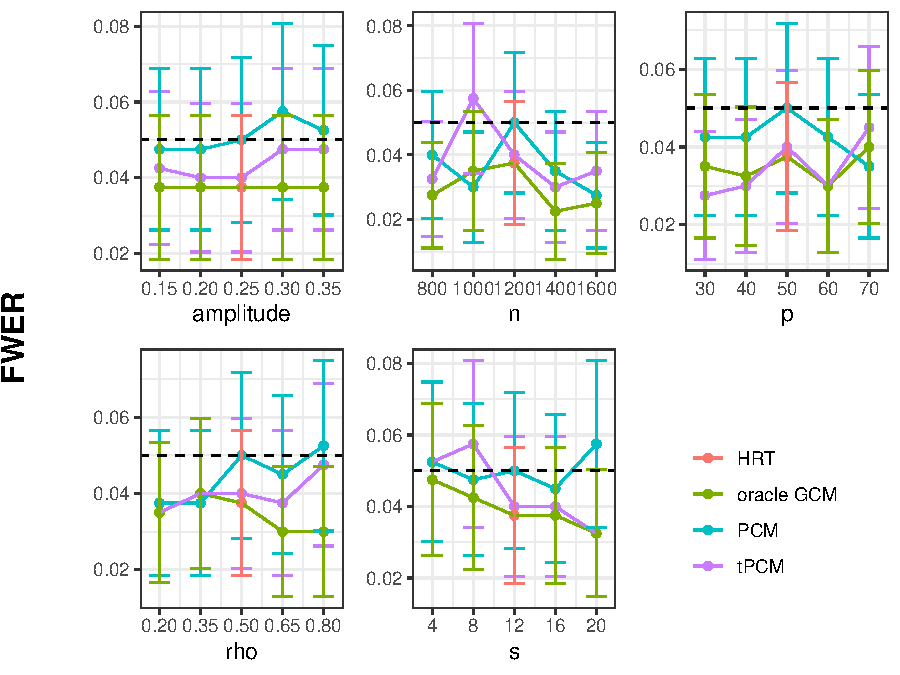
\includegraphics{figures/fwer_stat.pdf}
	\caption{Type-I error control: in each plot, we vary one parameter. Each point is the average of 400 Monte Carlo replicates, and the error bars are the average $\pm 2 \times \widehat{\sigma}_f$, where $\widehat{\sigma}_f$ is the Monte Carlo standard deviation divided by $\sqrt{400}$.}
	\label{fig:fwer}
\end{figure}

\section{Choosing the training proportions} \label{sec:choosing-training-proportions}
In this section, we justify our choice of the best training proportions for tower PCM and PCM. For tPCM, we compared training proportions in $\{0.3, 0.4, 0.5, 0.6, 0.7\}$. For PCM we compared training proportions in $\{0.3, 0.4, 0.5\}$. We plot the family-wise error rates and power for for each method in Figures \ref{fig:PCM FWER proportion}, \ref{fig:tPCM FWER proportion}, \ref{fig:tPCM power proportion}, and \ref{fig:PCM power proportion}. In terms of type-I error for tPCM, 0.7 seems the most conservative which is perhaps not surprising, as it uses more data for the nuisances and less for testing. The rest of the proportions do not follow a monotonic trend, however. Generally, all proportions seem to be controlling the type-I error, though 0.5 and 0.6 exhibit some slight inflation for some settings. The type-I error rate for PCM is also not monotone. It is unclear what we should expect, since smaller training proportion means more data for the in-sample fits on the test split, but a poorer estimate of the direction of the alternative on the training split. In terms of power, though there is not a single training proportion that dominates uniformly for both tPCM and PCM, 0.4 and 0.3 are generally the highest, respectively. 

\begin{figure}
	\centering
	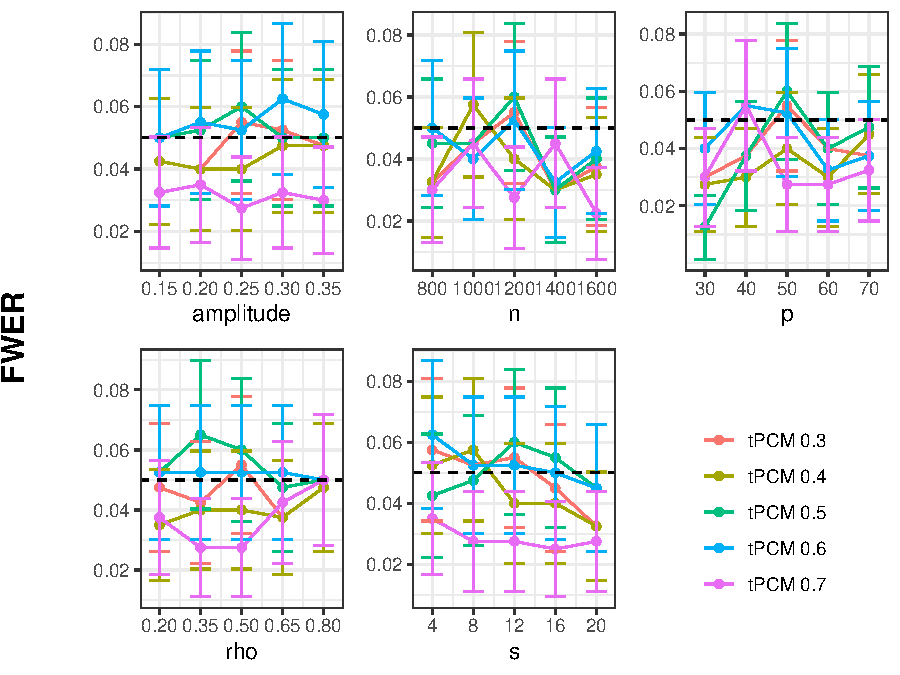
\includegraphics{figures/fwer_tPCM_choose_proportion.pdf}
	\caption{A family-wise error rate comparison of between  different training proportions for tPCM.}
	\label{fig:tPCM FWER proportion}
\end{figure}

\begin{figure}
	\centering
	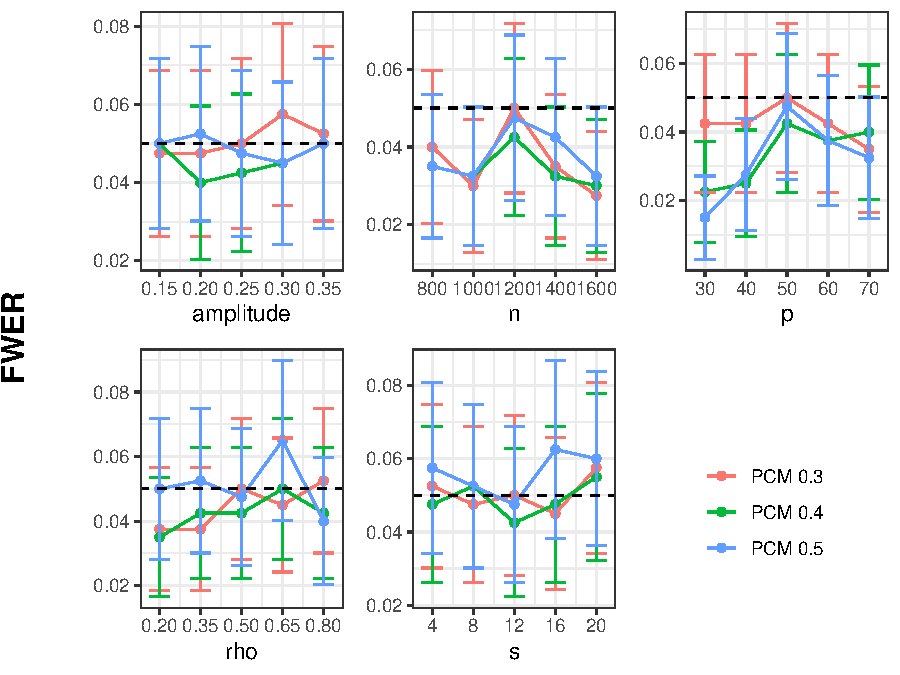
\includegraphics{figures/fwer_PCM_choose_proportion.pdf}
	\caption{A family-wise error rate comparison between different training proportions for PCM.}
	\label{fig:PCM FWER proportion}
\end{figure}

\begin{figure}
	\centering
	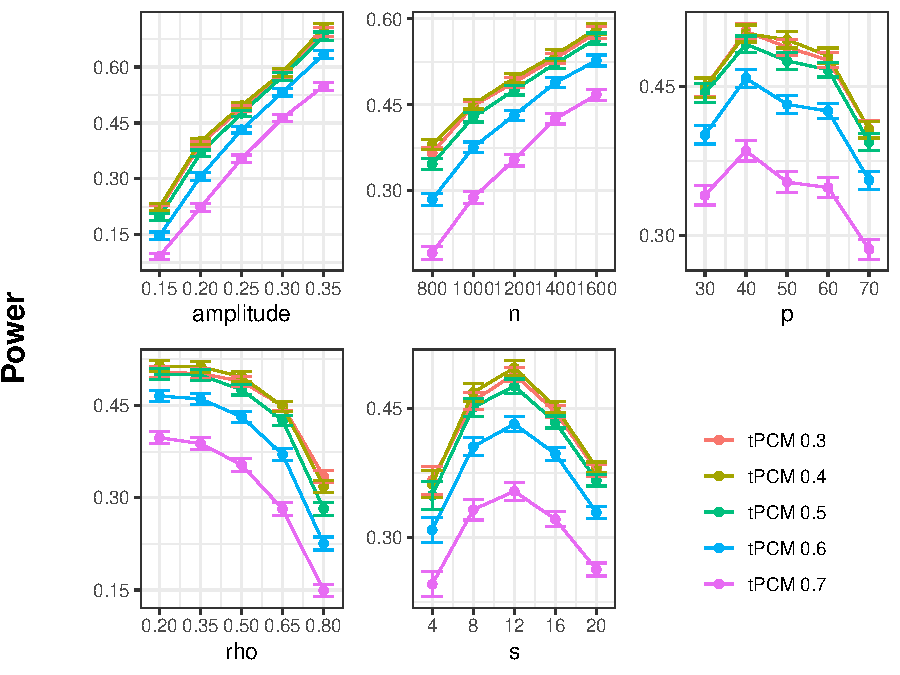
\includegraphics{figures/power_tPCM_choose_proportion.pdf}
	\caption{A power comparison between different training proportions for tPCM.}
	\label{fig:tPCM power proportion}
\end{figure}

\begin{figure}
	\centering
	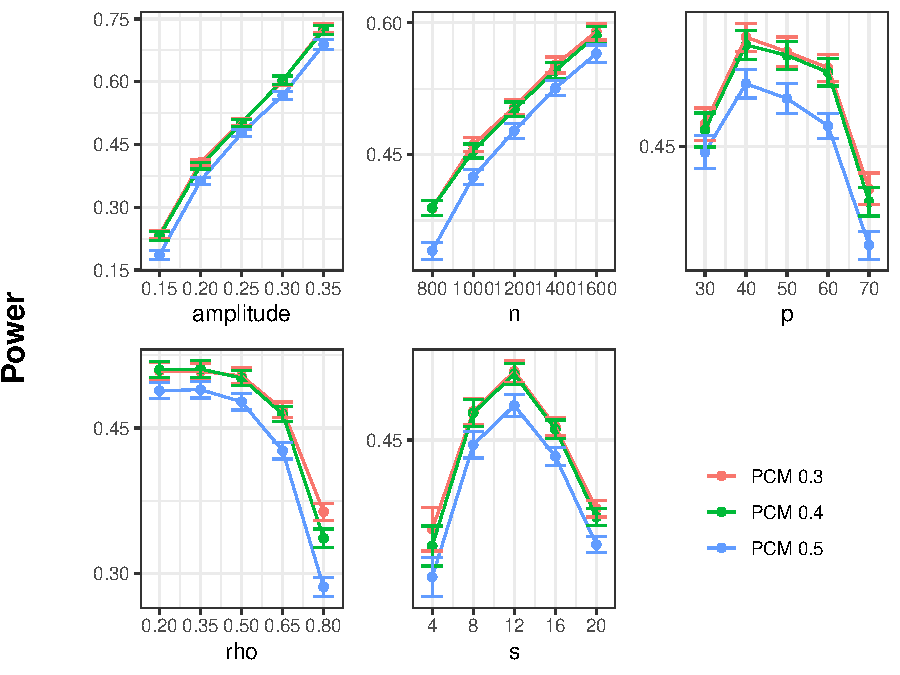
\includegraphics{figures/power_PCM_choose_proportion.pdf}
	\caption{A power comparison between different training proportions for PCM.}
	\label{fig:PCM power proportion}
\end{figure}

\section{Method implementation details in the data analysis} \label{sec:data-analysis-details}
\paragraph{HRT and tPCM}
HRT and tPCM utilized a 0.35 training proportion. On the training sample, we obtained fits for $\E[\pry \mid \prx]$ and $\law(\prx)$. For $\E[\pry \mid \prx]$, we used the same sparse GAM as implemented in the function \texttt{bam()} from \texttt{mgcv} with family = ``gaussian" and penalization parameter \verb|bs = "cs"|, as was done in our simulations. For $\mathcal{L}(\prx)$, we used the same fit as in \citet{Liu2020} and \citet{Li2021c}, which was the graphical lasso as implemented in the \texttt{CVglasso()} function from the \texttt{CVglasso} package with parameter \texttt{lam.min.ratio = 1e-6}. HRT utilized $B_{\text{HRT}} = 5000 \approx 3 \times p / \alpha$ resamples, and tPCM used $B_{\text{tPCM}} = 25$ resamples to approximate conditional means. 

\paragraph{PCM}
As in the simulation study, PCM was implemented as described in Algorithm 1 of \citet{Lundborg2022a}, except for Step 2, so it included the extra step (1(ii)) that can be performed when the contribution to $\E[\pry \mid \prx]$ from $\prx_j$ can be separated from the contributions from the other predictors, as is the case with a GAM. PCM also used a 0.35 sample split, and also used the sparse GAM implentation from the \texttt{bam()} function with family =``gaussian" as in the previous methods for fitting $\E[\pry \mid \prx]$ on the training split, as well as for fitting $\E[\pry \mid \prx_{\minus j}]$ and $\E[f_j(\prx_j) \mid \prx_{\minus j}]$ on the evaluation split. A significant distinction from the simulation setting was that there is no banded structure with a known bandwidth of 1, so the regression of $f_j(\prx_j)$ on $\prx_{\minus j}$ had to include all of the $p - 1$ predictors in $\prx_{\minus j}$, rather than just $\prx_{j-1}$ and $\prx_{j+1}$. 

\paragraph{tGCM}
tGCM is akin to the oracle GCM from the simulation, except $\E[\pry \mid \prx]$ and $\law(\prx)$ are estimated from the data. tGCM uses the same tower-based acceleration as the tPCM test. There is no danger of a degenerate limiting distribution under the null, so we can make use of the full sample for testing through 5 fold cross-fitting. For each of the five equally sized folds, $\E[\pry \mid \prx]$ and $\law(\prx)$ are estimated on the remaining 4/5 of the data using the same estimators as for HRT and tPCM. The tower trick is utilized to estimate $\E[\pry \mid \prx_{\minus j}]$ from the estimates for $\E[\pry \mid \prx]$ and $\law(\prx)$ using 25 resamples.
\end{document}



